\documentclass[openany]{book}
\usepackage[utf8]{inputenc}
\usepackage{graphicx}
\usepackage{amsmath}
\usepackage[a4paper, total={6in, 8in}]{geometry}
\usepackage{booktabs}
\usepackage{caption} 

\captionsetup[table]{skip=5pt}

\renewcommand{\baselinestretch}{1.5}

\title{Learning Depth and Visual Odometry From Light Fields \\
\large AMME4111 Thesis A Progress Report}

\author{Joseph Daniel}
\date{November 2019}

\begin{document}

\maketitle

\tableofcontents

\chapter{Introduction}
Humans have a remarkable ability to perceive visual stimuli emanating from the world around them. Not only do we identify different objects, scene depth, movement, and colour with ease, but we often draw meaning and even enjoyment from the combination of light rays bouncing around space and arriving at our eyes. Man-made machines on the other hand are much more easily decomposed into a set of deterministic modules that require explicit, well defined instruction sets. This thesis is concerned with developing a set of algorithms that breaks down, and utilises the wealth of information in image data to produce valuable signals that can be employed in robotic perception. 

\section{Motivation}
True autonomy in mobile robotics requires the ability to perceive the world adequately. In particular, understanding the structure and size of the space inhabited by the robot, as well as its own movement through that space are vital to its ability to navigate and interact with the world. Computer vision algorithms in combination with increasingly lower-cost and higher quality imaging hardware offers a popular solution, encompassing enormous diversity in sensing modalities and precipitating the development of powerful perception systems in modern robotics. Plenoptic imaging is one such expression of evolving imaging technologies that continues to yield promising results in tasks such as mapping \cite{kuehefuss2016rgbdslam}, underwater imaging \cite{skinner2016underwaterplenoptic}, low light imaging \cite{dansereau2015volumetric}, and classification \cite{wang2016lfcnn}.

This work is concerned with the application of \textbf{plenoptic imaging} in two intimately related tasks: \textbf{visual odometry} which involves estimating the motion of a camera in 3D space, and \textbf{depth reconstruction} which estimates the shape of the scene in an image. One might question the practicality of using image data for these tasks when great success has been found with more specialised sensing modalities; motion estimation for example is typically addressed with inertial navigation systems or global positioning system (GPS) receivers. Other robotic systems employ lidar, acoustic range-finding, time-of-flight cameras or structured-light cameras to gain access to 3D models of the scene inhabited by the robot. 

Cameras however, can often offer superior qualities in size, weight, cost, power consumption, and they deliver a rich, highly detailed representation of the world. Furthermore, unlike \textit{active} sensor technologies which sense the world by 'illuminating' it, cameras are \textit{passive} sensors, meaning they do not interfere with one another and can be used outdoors, in the vacuum of space or underwater. Thanks to their ability to adjust their exposure period, aperture size and sensor gain, cameras are also highly capable in a variety of lighting conditions and environments, independent of the medium in which they operate.


\section{Problem Statement}
Humans are exceptionally well adapted to these tasks - our two eyes allow us to process the 3D geometry of the scene, while our learned experiences are often able to fill in the gaps where geometric information is insufficient or unavailable. Image processing algorithms are not equipped with this same kind of human intuition, and so the deceptively complex task of estimating the 3D structure of a scene from a sequence of images continues to attract attention from the computer vision community \cite{dansereau2011plenopticflow,nister2004vo,gakne2018scale,zhou2019scale}. 

The price of camera components is decreasing while image quality continues to improve, not only making cameras an attractive perception module for autonomous robotics, but also spurring the popularity of multiple-view imaging. Embracing this idea, this work develops an algorithm that performs these tasks by taking advantage of the rich geometric information exposed when using multiple views. Thus, the vocabulary and concepts from the literature on light field imaging are adopted broadly throughout this work. More broadly however, the principle underpinning much of this thesis is that novel imaging devices that break away from the traditional pinhole model of the camera have vast implications in the field of machine vision. We need not look any further than the animal kingdom to see why this is true - the biological eye is estimated to have evolved independently no fewer than 50 times, each variant acutely adapted to the particular set of challenges in their environment. The diversity and evolutionary ingenuity in biological visual perception systems prompts an important question in robotics and computer vision - how best should we equip robots to see the world given a particular set of challenges and environments? In this thesis, a camera array which is a simple yet versatile extension of the stereo camera is used to develop the algorithms that address the visual odometry and depth reconstruction problems. 

While there are well established solutions addressing these tasks, an important contribution of this work is the idea of 'self-calibration'. Robots operating in challenging environments are frequently subjected to destabilising effects such as thermal expansion, vibration and shock, rendering precise equipment calibrations invalid. Multiple-view geometry is materially dependent on the orientation and position of the cameras; rotating a camera even a few arc-seconds from its calibrated position results in a disproportionally magnified error in the image being formed, especially in large, open spaces. A self-calibrating and adaptive perception module which is robust to these effects is therefore an attractive capability in robotics. The self-calibration problem is addressed in this thesis with the use of data-driven models that learn directly from experience in an unsupervised manner. Unsupervised machine learning makes 'online-learning' possible, in which models take advantage of new data becoming available in-situ, improving performance and building robustness to different environments. Most importantly however, unsupervised models are able to adapt to errors in the calibration of the equipment without requiring hand-labelled data to supervise the learning process. Furthermore, data driven models are able to build robustness to situations that are difficult to hand-craft solutions to, such as foggy weather, rain, and reflective surfaces.

\section{Outline}
Concepts from computer vision, machine learning and light field imaging are used heavily throughout this thesis, and \textbf{Chapter 2} begins by providing an overview of the relevant background information. On the subject of computer vision, it describes the pinhole model of the camera, the fundamentals of multiple view geometry, and develops intuition relevant to light field imaging. Machine learning is presented as an approach to solving computer vision problems, with emphasis directed towards convolutional neural networks, as an algorithm that continues to gain popularity in image based problems.

The existing approaches for performing visual odometry and depth estimation are reviewed in \textbf{Chapter 3}, presented in two categories: geometric approaches which rely on directly modeling movement through 3D space, and machine learning approaches which take advantage of massive datasets to build resilient, data-driven solutions.

\textbf{Chapter 4} introduces a novel light-field based algorithm for simultaneously learning depth and pose. Though algorithms have been proposed in previous work that perform the two tasks either monocularly or with stereo camera pairs, this thesis differs in the use of light-field imagery to gain improved access to geometric information in the scene. While previous work has benefitted from large scale open source datasets, similar pose-stamped footage does not exist publicly for camera arrays. The acquisition of such a dataset thus forms one of the objectives of this thesis, the methodology for which is discussed in the chapter.

\textbf{Chapter 5}, presents the results from initial experiments using the pipeline described in chapter 4, performed on both the early dataset and the open source KITTI dataset \cite{dataset-kitti}. The early challenges and milestones are discussed, and a qualitative discussion on the successes, failure modes, and future directions is presented. 

An updated research proposal is provided in \textbf{chapter 6} with emphasis placed on the expected milestones in the remainder of the project. 




\chapter{Background}

\section{Geometry in Computer Vision}

The pixel is the building block of digital imagery. Thanks to our ability to fabricate advanced circuits on the scale of nanometers, digital camera sensors have become ubiquitous - making their way into all manner of consumer devices. Because the photodiodes in camera sensors are typically arranged on a 2D plane, most of our operations on digital images manipulate the 2D structures present in that pixel data. However, it is important to remember that the 2D shapes and structures that appear on the sensor plane are projected versions of a 3D world. 

\subsection{The Pinhole Camera}

The most basic kind of camera, the pinhole camera projects a 3D world point $[X, Y, Z]$ to a homogenous coordinate on a 2D plane $[u, v, w]$. This relationship is captured in the $3 \times 3$ camera intrinsics matrix \cite{szeliski2010computervision}, and is typically written as 

\begin{equation}
\begin{bmatrix}
    u\\
    v\\
    w
\end{bmatrix} = 
\begin{bmatrix}
    f_x & s & u_0 \\ 
    0 & f_y  & v_0 \\ 
    0 & 0 & 1 
\end{bmatrix}
\begin{bmatrix}
    X \\
    Y \\
    Z
\end{bmatrix}.
\end{equation}

The intrinsics matrix can alternatively be thought of as mapping ray directions to pixel coordinates:

\begin{equation}
\begin{bmatrix}
    u\\
    v\\
    1
\end{bmatrix} = 
\begin{bmatrix}
    f_x & s & u_0 \\ 
    0 & f_y  & v_0 \\ 
    0 & 0 & 1 
\end{bmatrix}
\begin{bmatrix}
    tan(\theta) \\
    tan(\phi) \\
    1
\end{bmatrix}.
\end{equation}


\begin{figure}[htbp]
    \centering 
    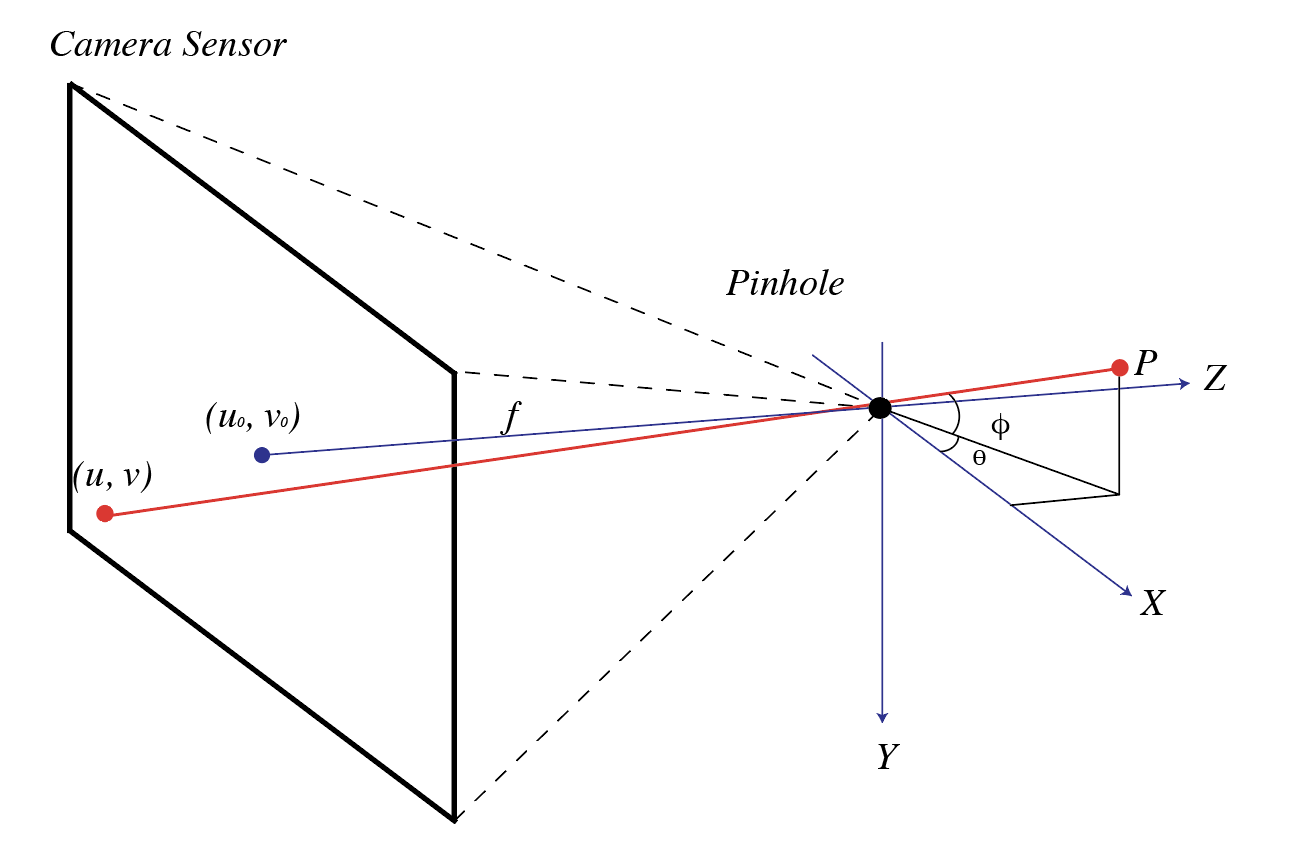
\includegraphics[width=4in]{images/pinhole.png}
    \caption{The pinhole model describes how a light ray originating from world coordinate $P$ is received at pixel coordinate $(u, v)$. Equivalently, the pinhole model can be thought of as associating the light ray of elevation $\phi$ and azimuth $\theta$ with the specific pixel coordinate $(u, v)$. Since the relationship is a one-to-one mapping between ray directions and pixel coordinates, the inverse of the intrinsics matrix $K^{-1}$ associates each pixel with a corresponding ray direction.}
\end{figure}



\subsection{Epipolar Geometry and the Fundamental Matrix}

Epipolar geometry describes the relationship between two cameras, and imposes a set of constraints which makes it possible for us to draw meaningful geometric information when we have two views of the same scene. This relationship is encapsulated in a $3 \times 3$ matrix called the Fundamental matrix $F$. The culmination of the epipolar constraint is that any point in 3 dimensional space that appears at pixel $(u_1, v_1, 1)$ in one view and $(u_2, v_2, 1)$ in the second view must satisfy the relationship:

\begin{equation}
    \begin{bmatrix}
        u_1, v_1, 1
    \end{bmatrix}^T
    F
    \begin{bmatrix}
        u_2, v_2, 1
    \end{bmatrix}
    = 0.
\end{equation}

\begin{figure}
    \centering
    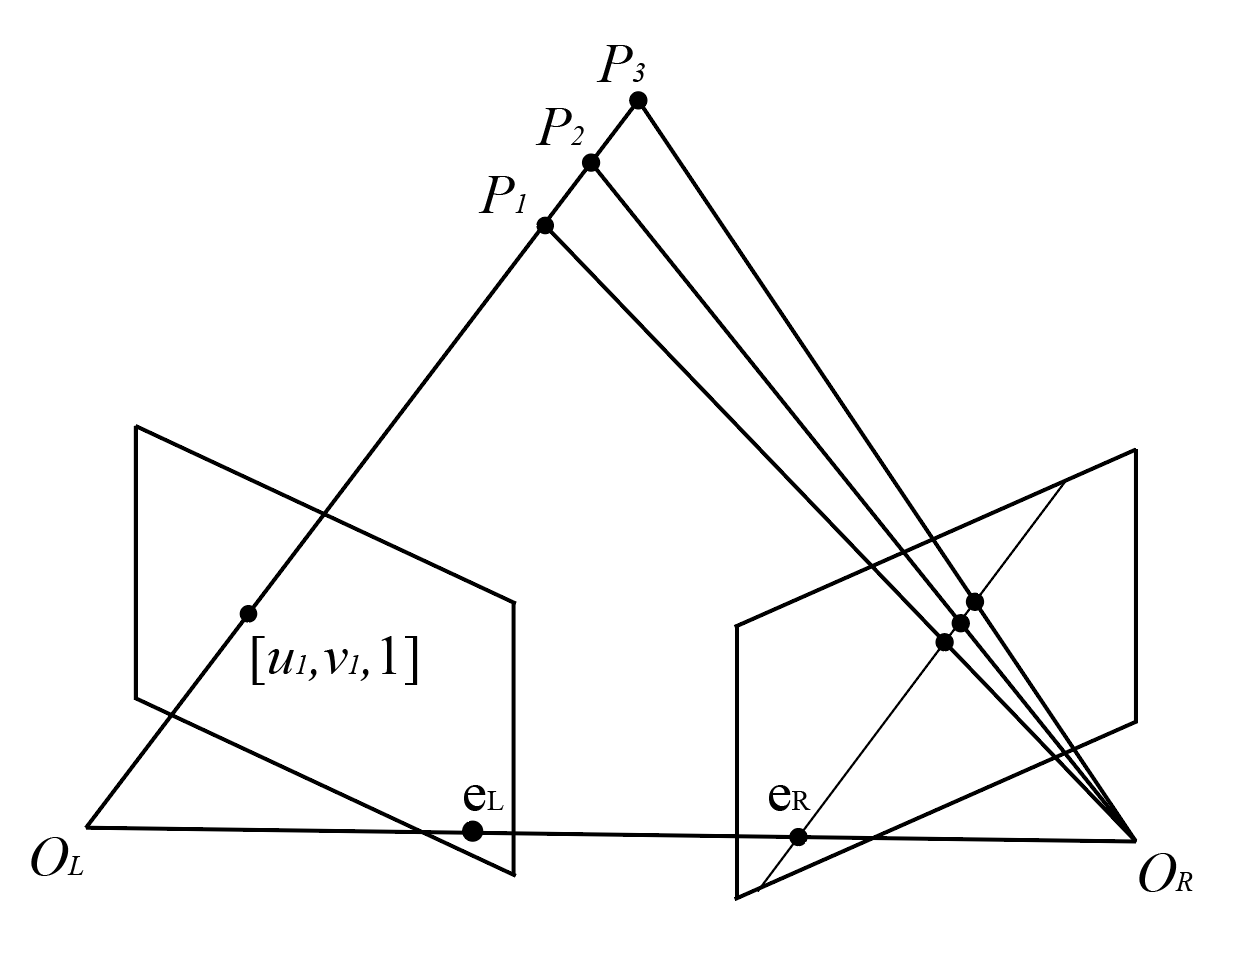
\includegraphics[width=2.5in]{images/epipolarplane.png}
    \caption{Epipolar geometry is the geometry of stereo camera pairs. Without knowing depth, the point $[u,v,1]$ can be projected to any number of points $P1, P2, P3... $ in 3D space, having many possible projections on the sensor plane of the right camera. The Fundamental matrix however constrains the set of possible projections to lie on a straight line called the epipolar line.}
    \label{epipolarplane}
\end{figure}

The Fundamental matrix thus describes the rotation and translation between two cameras up to scale. Any point projected from pixel coordinate $[u_1, v_1, 1]$ must lie on the epipolar line in the second image, which is formed by the intersection of the epipolar plane and the imaging plane. 



\section{The 4D Light Field}
Light field imaging has emerged as a powerful tool in computer vision for robotics, offering a rich higher-dimensional representation than what can be captured by conventional optics. The underlying principle used to describe the light field is the plenoptic function, a 7-dimensional mapping that assigns radiance values to the light rays at every position in space, in every orientation, at all wavelengths, throughout all of time \cite{adelson1991plenoptic}. This can be formally expressed as $L(x,y,z,\theta, \phi, \lambda, t)$, and measured in $W/m^2/sr/nm/s$. 


Levoy et al. \cite{levoy1996lfrendering} shows that with the addition of practical constraints however, the plenoptic function can be expressed more concisely as a parameterisation of 4 variables. Pixels on camera sensors integrate the number of photons arriving at them over a finite period of time removing the temporal dimension, and each colour channel can be thought of as a monochromatic sampling of the light field, removing the spectral dimension. Additionally, and importantly, is the constraint that the radiance of light rays propagating through a vacuum do not change if samples are restricted to the convex hull of the scene, thus reducing the overall dimensionality of the plenoptic function by one parameter \cite{levoy1996lfrendering}. To illustrate this, one could think of the light rays leaving the inside of a bowl sat upright on a table. Many of those rays may only travel a small distance before being blocked by the inside of the bowl itself, meaning those rays will never be registered by any practical measurement device. As shown in Figure 2.3 if we consider only the convex hull of the bowl however, we are required only to represent the value of the plenoptic function on the encapsulating surface of the object \cite{gortler1996lumigraph}.

\begin{figure}[htbp]
    \centering
    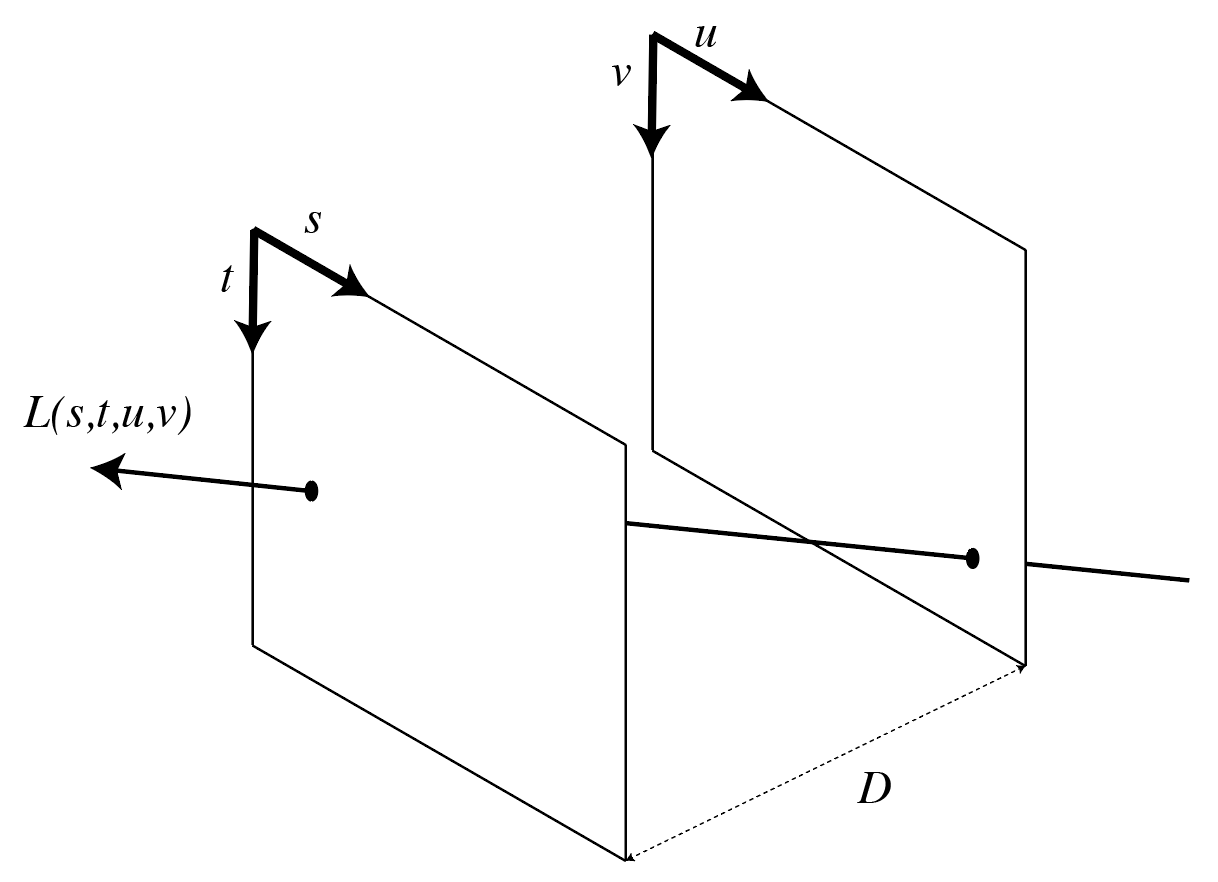
\includegraphics[width=2.5in]{images/2pp.png}
    \label{convexhull}
    
\includegraphics[width=0.3in]{images/blank.png}
    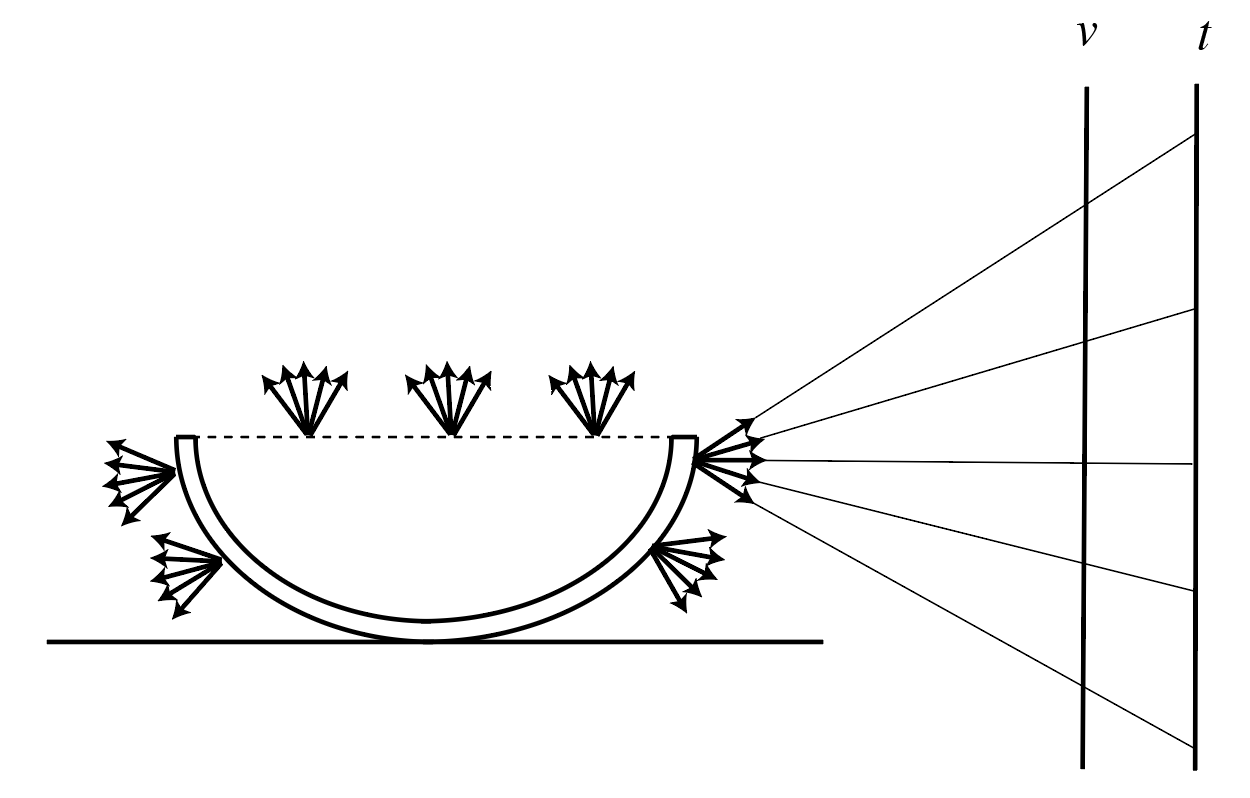
\includegraphics[width=2.5in]{images/convexhull.png}
    
    \caption{Two plane parameterisation (left): the plenoptic function can be described by the radiance along a ray passing through two parallel planes. The free space assumption (right): if we consider only the bundle of rays leaving from the convex hull of the object at a particular instance in time, in a single colour channel, we can parameterise the light rays as a function of 4 variables rather than 7.}
    
    
\end{figure}

Also illustrated is a common convention for describing light rays in this 4 dimensional space called the two plane parameterisation \cite{gortler1996lumigraph}. In this parameterisation, two parallel planes are used to fix both the position and orientation of each ray by fixing their points of intersection with two parallel planes. By convention, the plane closest to the scene is termed \textit{u, v} and the plane closest to the camera sensor is the \textit{s, t} plane.

This 4D realisation of the light field originated as a model of rendering 3D computer graphics, one which shifted emphasis from notions of texture and geometric primitives to modeling the behaviour of light rays permeating space. Since then however, the conceptual framework of the light field has drawn a following of researchers at an intersecting region of signal processing, computer vision and robotics \cite{dansereau2014phd}. This notion of light field imaging finds a foothold in this work through the utilisation of camera arrays, which are devices that sample multiple views of the same scene. Using a camera array is a simple method for acquiring a sparse sample of the light field, where the position of the camera determines \textit{(s,t)} while the location of the pixel determines \textit{(u, v)} \cite{yao2016camarray}. The images captured from a camera array are mapped easily to the 4D light field, and identifying corresponding pixels across images exposes a rich tapestry of geometric information about the scene. 


\begin{figure}[tbp]
    \centering
    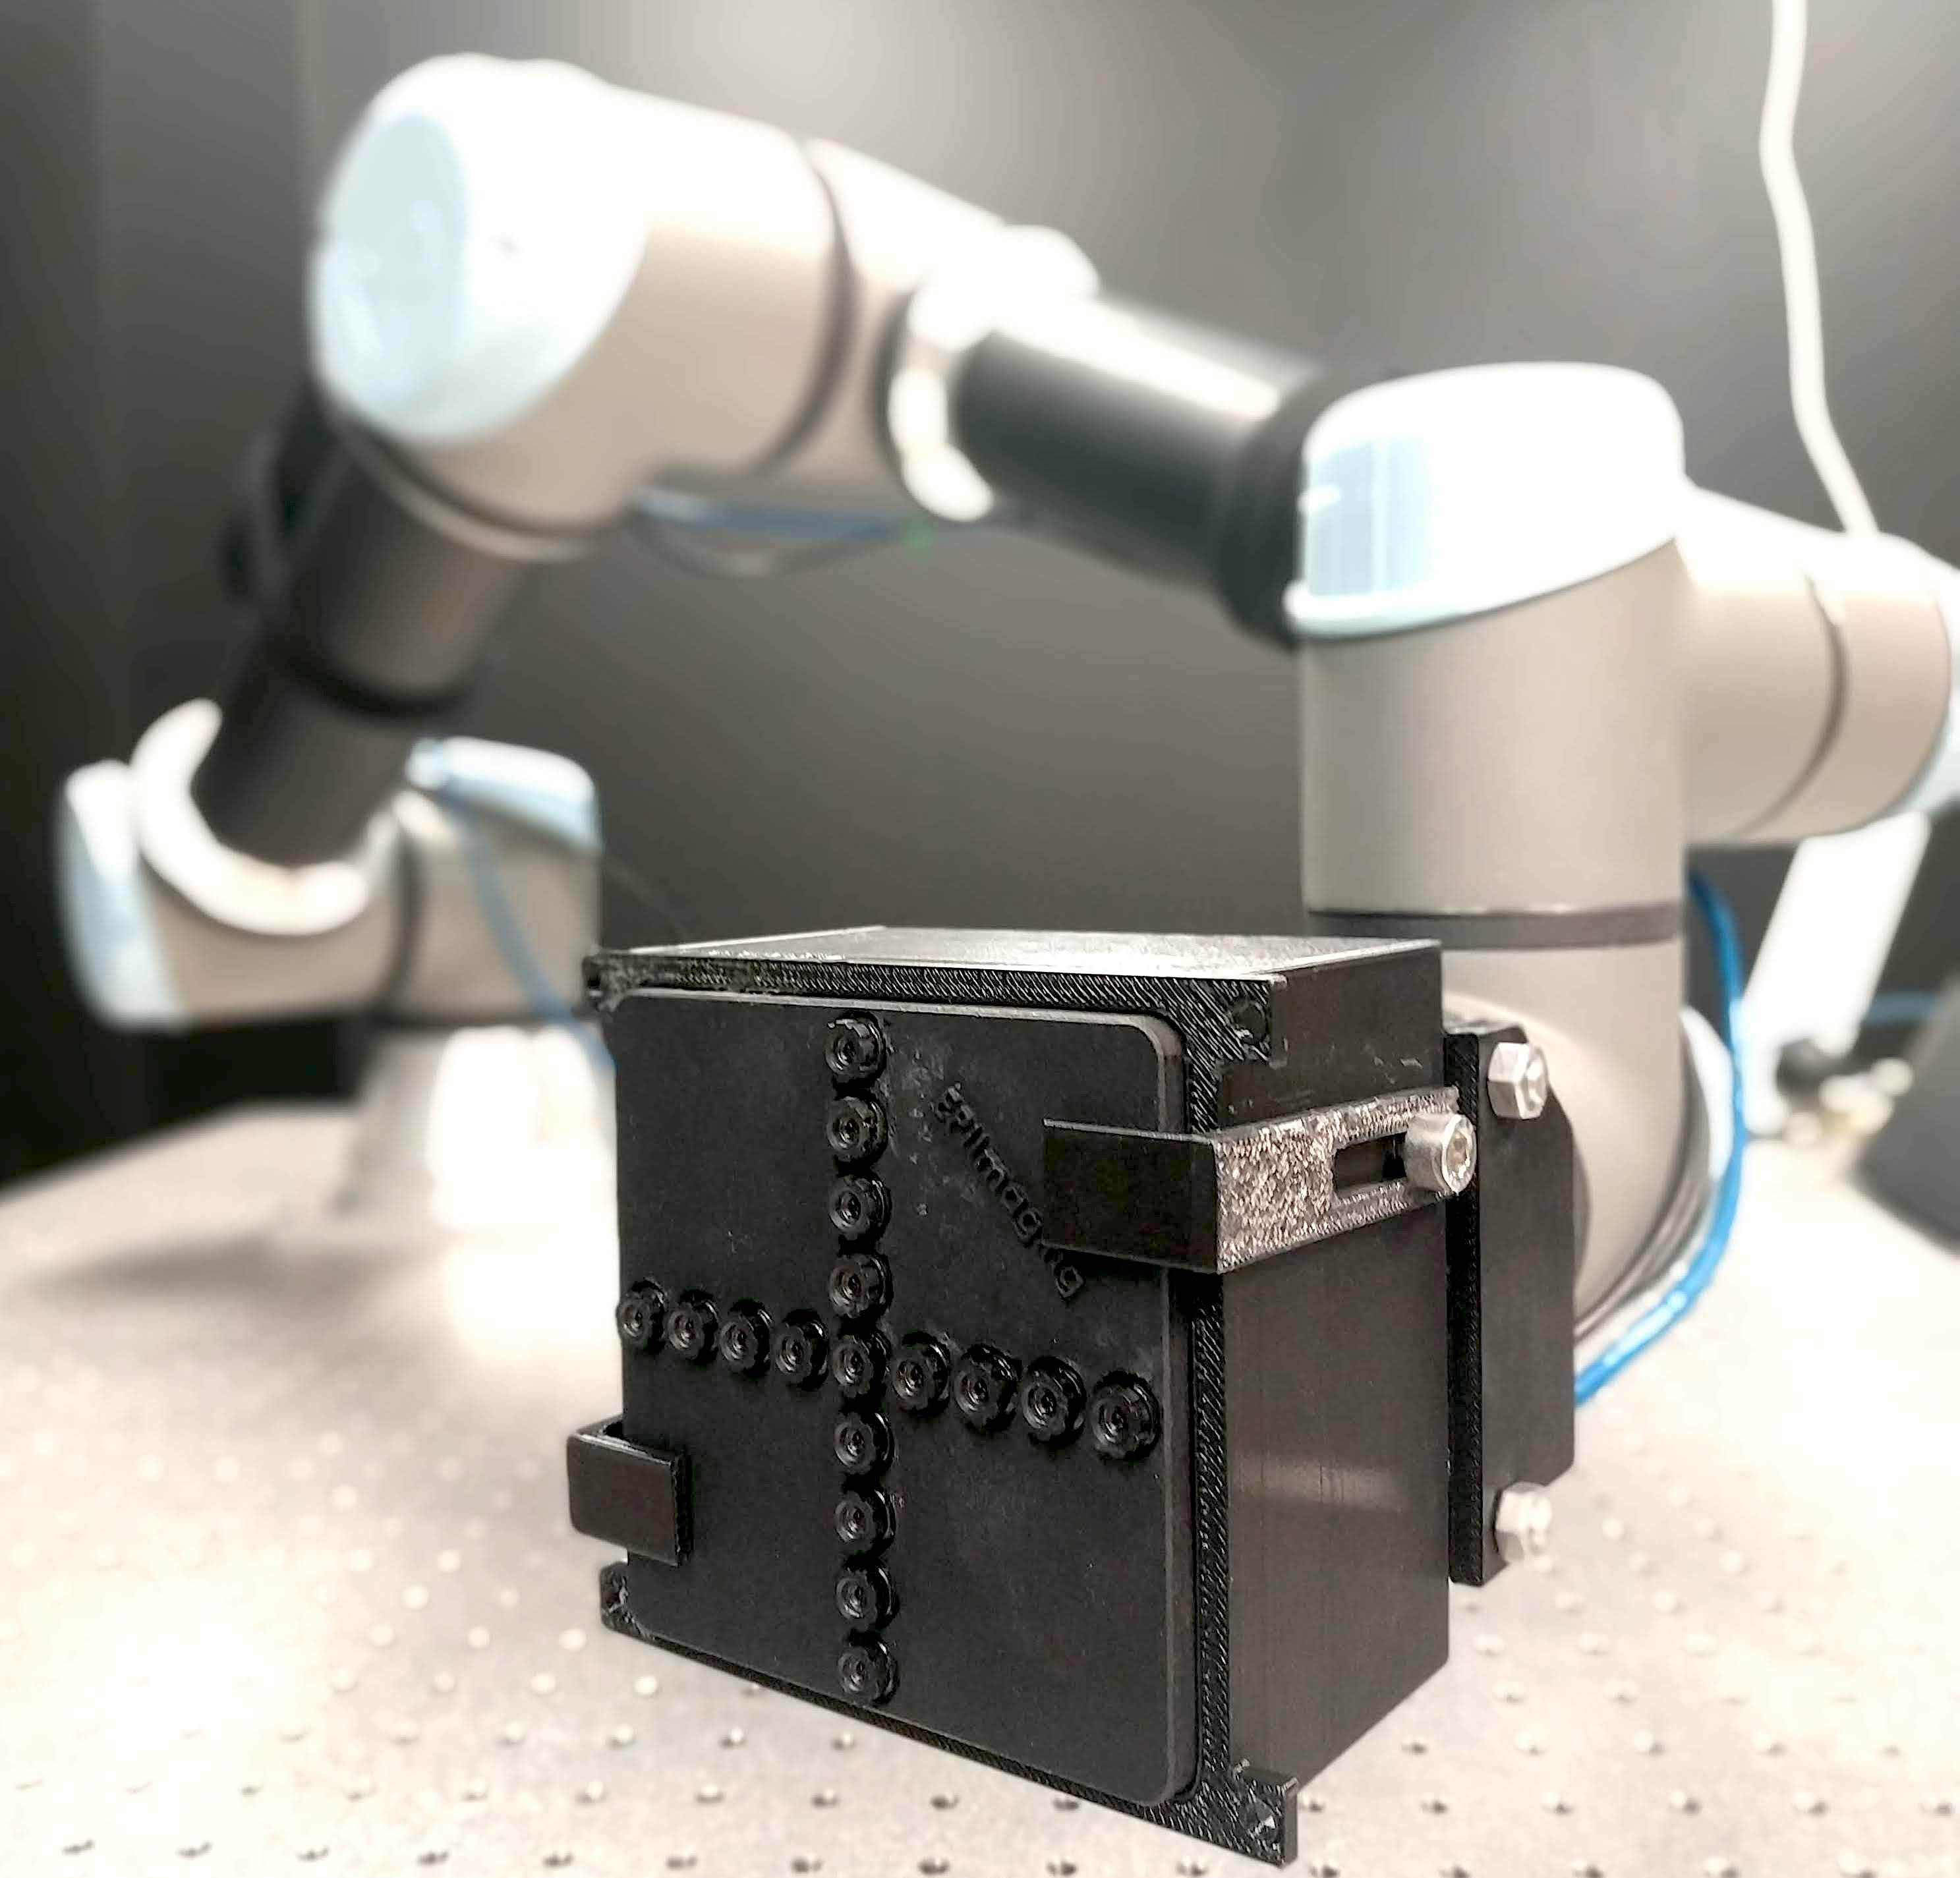
\includegraphics[width=4.5in]{images/robotcamera.jpg}
    \caption{An example of a camera array mounted on a robotic arm. This camera array is configured as 17 sub-apertures arranged on a single plane in a cross-hair formation. Camera arrays sample several views of the same scene and are thus capable of acquiring a sparse sample of the light field. This is the camera that will be used throughout this thesis project.}
    \label{cameraarray}
    \vspace{1cm}
    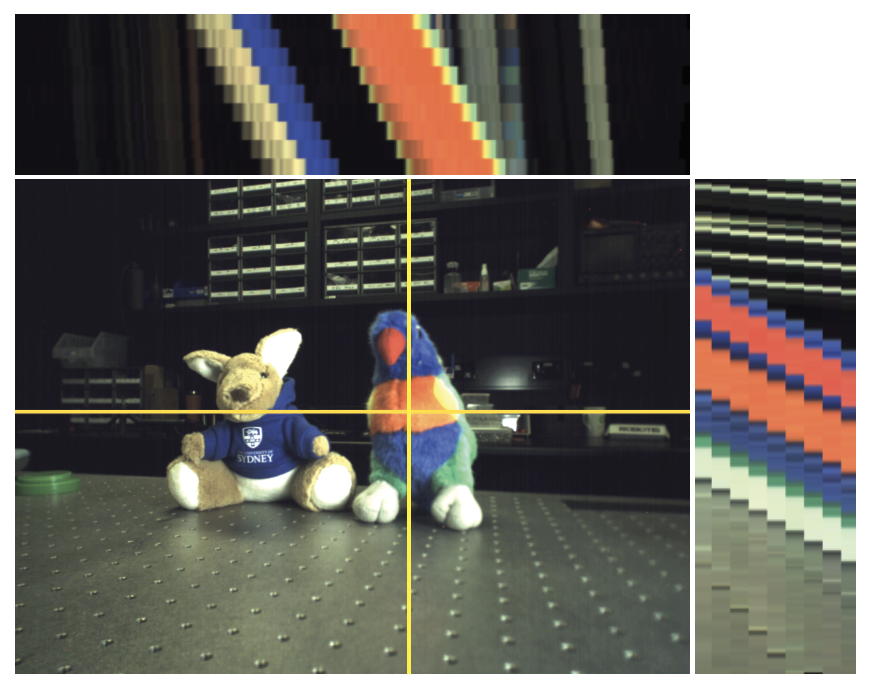
\includegraphics[width=2in]{images/epipolarimage.png}
    
\includegraphics[width=0.4in]{images/blank.png}
    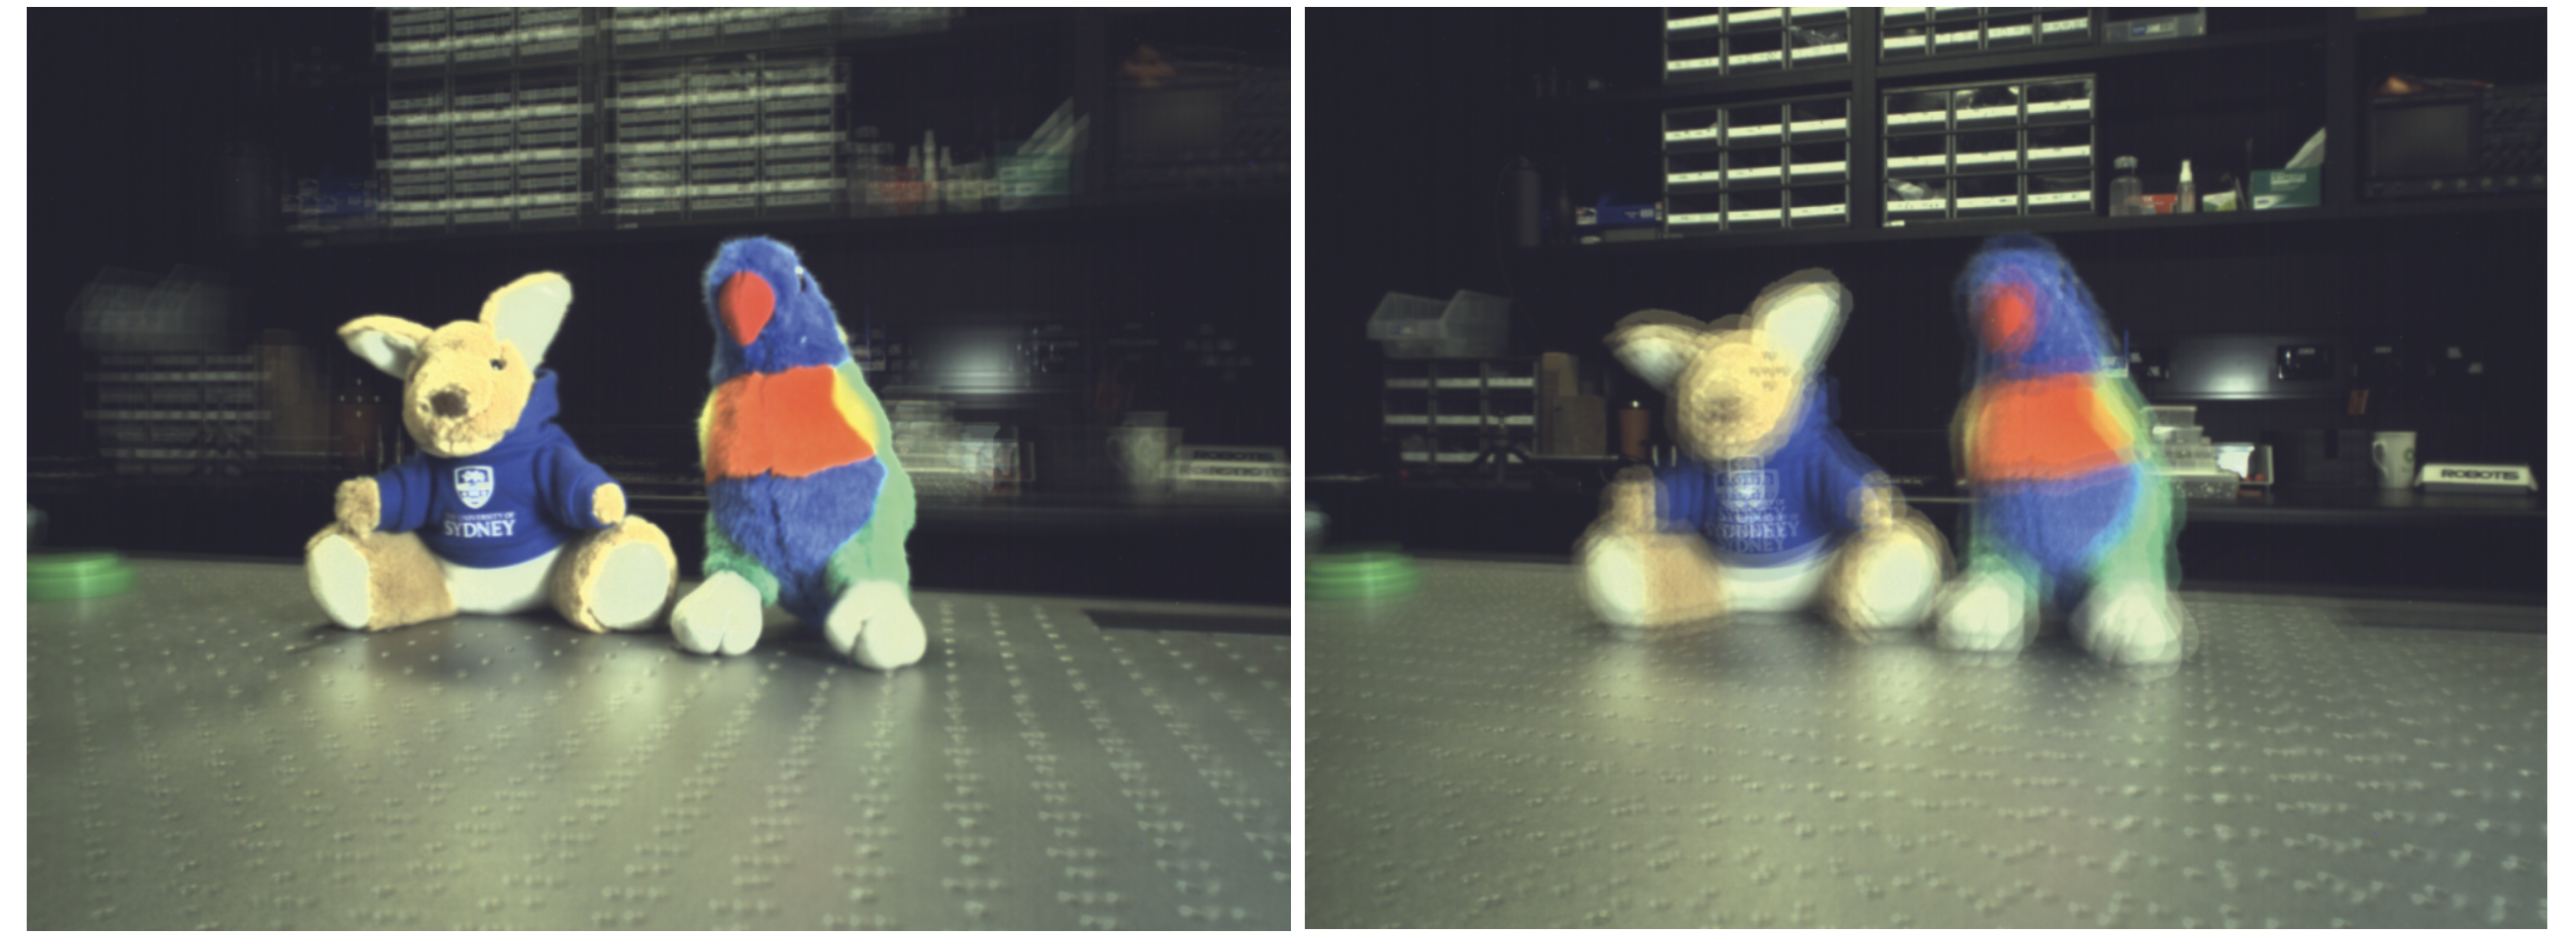
\includegraphics[width=3.5in]{images/refocus.png}
    \caption{Epipolar Plane Images (left): Shown as a slice of a volume, the images formed by dissecting the image in the \textit{s,u} and \textit{t,v} planes are characterised by sheared straight lines, with the grade of the slope encoding the amount of parallax experienced by a pixel at that \textit{u} or \textit{v} coordinate. Synthetic aperture focusing (right): taking the average of every image from the camera array yields an image where different parts are in focus depending on the alignments of the images.}
    \label{epiplaneimg}
\end{figure}


One way that this geometric information can be easily visualised is by taking slices of the light field image in the \textit{s,u} or \textit{t, v} axes as shown in Figure \ref{epiplaneimg}. While the idea of taking a 2D slice from the 4D image can seem complex, the task of generating a so called 'epipolar plane image' from a camera array is deceptively simple. Images captured from camera arrays can be stacked to form a solid volume, from which 2D slices can be sampled. Each of these slices yields an image characterised by sheared straight lines, encoding information about the geometry of the scene, including depth and occlusions \cite{bolles1987epiplane}. 

The geometric information encoded in a light field sampling can alternatively be visualised by processing the image into a 'focal stack'. Focal stacks closely resemble images with shallow depth of field such as those that can be captured from a commercial DSLR camera. Light field focal stacks differ from focus in the optical sense however in that they are synthetic and can be recomputed after the image has been taken, effectively allowing control over the depth of field and focal depth in post-processing. Focal stacks can be computed from camera array images by layering images over one another and taking the average value for each pixel. The result is that parts of the scene that closely overlap appear in focus while areas with poor overlap create a 'bokeh' effect. More formally, if the relative pose of each camera is known, a specific focal stack for any desired depth can be computed by projecting each image onto the desired focal plane, and computing their average \cite{vaish2004parallax}.

These representations of the light field play an important role in this thesis project as we experiment with different methods for feeding light field images to the machine learning pipeline. An important consideration in any machine learning algorithm is the feature space - based on what particular inputs will the algorithm be making its decision? Raw images contain millions of measurements and thus represent an incredibly high-dimensional feature space for neural networks to process. Light field images are several times larger, and thus it is important that some form of dimensionality reduction is used to ease the training process. With the goal of investigating effective methods of feeding light fields to neural networks, this thesis will explore the use of three different light field formats as the entry point to the machine learning pipeline. The first two will be the focal stack, and epipolar plane image described above, interpreting the images as a 3 dimensional volume created by stacking 2 dimensional images on top of one another. The third will treat the light field as a 4 dimensional volume, requiring a 4D signal processing pipeline to fully take advantage of the dimensionality.

\section{Machine Learning in Computer Vision}


An oft-quoted anecdote in computer vision tells of MIT researcher Seymour Papert, who in 1966 assigned a summer project that sounded simple enough, namely to construct a 'visual system' that could describe what objects it saw by name \cite{papert1966vision}. While the regimes of computer vision have evolved substantially since 1966, many of the ideas, and challenges have persisted. This is embodied in the popularity of projects such as the ImageNet Large Scale Visual Recognition Challenge (ILSVRC) \cite{ilsvrc}, drawing researchers from institutions around the world. It was at the ILSVRC annual challenge where in 2012, a convolutional neural network achieved a top-5 error rate of 15.3\%, outperforming all previous submissions by 10.8\% \cite{krizhevsky2012alexnet}. Until 'AlexNet' in 2012, the competition consisted of competitors introducing algorithms that produced marginal improvements year on year. Needless to say, an improvement of over 10\% generated noise in the computer vision community, drawing attention to the powerful capabilities of deep learning.

While deep neural networks for computer vision have gained massive popularity since the success of AlexNet, the history of neural architecture models begins much earlier, with the perceptron as described by Frank Rosenblatt in \cite{rosenblatt1959neurodynamics}. The fundamental building block of neural networks, the 'perceptron' is a module that accepts several inputs, and produces a single output computed as a weighted sum of each input - allowing complex functions to be approximated when several perceptrons are layered together as a 'multilayer perceptron' \cite{minsky1969perceptrons}. The process of finding the optimal set of weights that produce the desired output given a set of inputs is referred to as training, and in practice is usually found by optimising some cost function using the backpropagation algorithm \cite{rumelhart1986backprop}. Backpropagation uses the chain rule of calculus to calculate partial derivatives of each weight in the network with respect to the cost function. A gradient based optimisation algorithm such as stochastic gradient descent (SGD) can then be employed to minimise the cost function. Thus, it is important that each step in the computation of a neural networks output be differentiable - that is, it must support the backpropagation of gradients or else gradient-based optimisation will fail.

\begin{figure}[tbp]
    \centering
    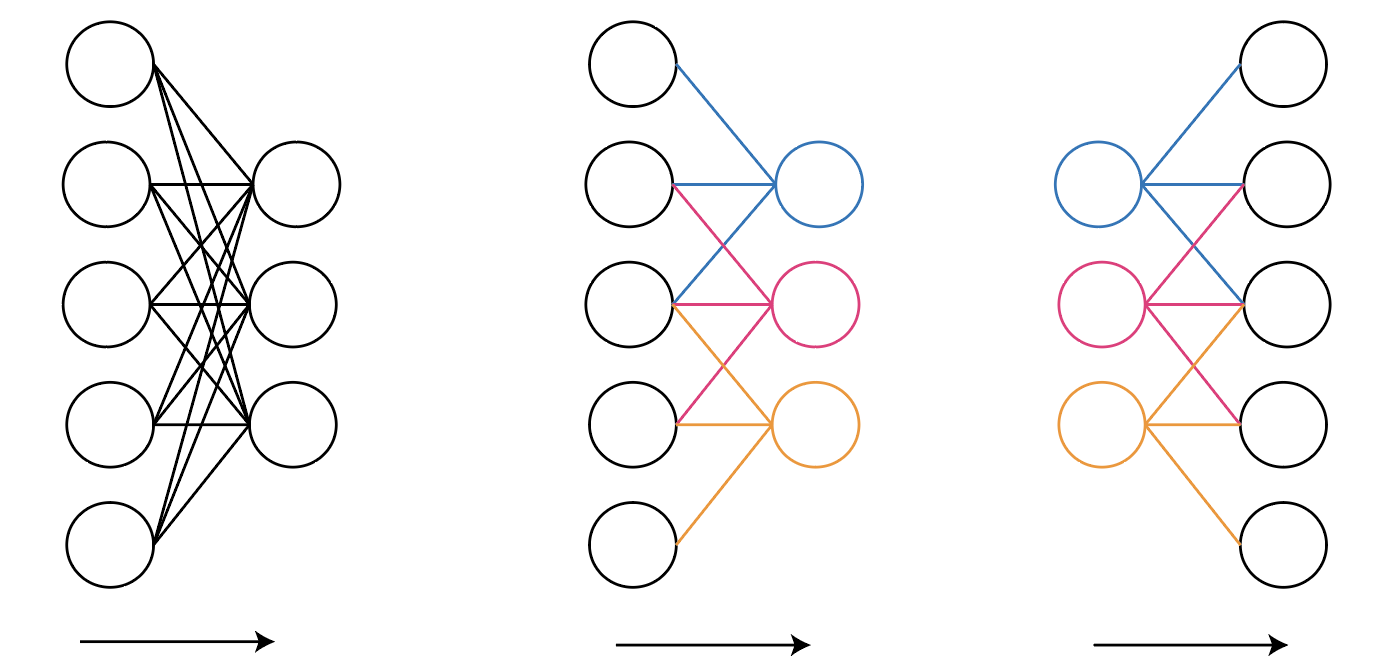
\includegraphics[width=5in]{images/cnnvsmlp.png}
    
    \caption{Multilayer Perceptron (left): each output from one layer is fed into the inputs of every node in the subsequent layer. Convolutional Neural Networks (middle) on the other hand have a 'receptive field', taking advantage of the spatial coherence of pixels in image data. The convolutional upsampling operation (right) is frequently used to upsample a low-dimensional feature space, to a higher dimensional one. It is often employed as a 'learned' information decompression.}
    
    \label{convexhull}
\end{figure}


Convolutional neural networks (CNN's) are similar to multilayer perceptrons, but introduce a spatial invariance that makes them particularly well suited for extracting high-level features from image data. Where multilayer perceptrons are densely connected, the connectivity pattern of each node in a CNN takes advantage of the hierarchical organisation of patterns in image data by using a 'receptive field'. Biologically inspired, these nodes respond to stimuli only in their receptive field, and so they typically learn to identify salient 'features' in the image - combinations of pixels that represent some kind of underlying structure. As these types of networks grow deeper, the features that they learn typically become more complex \cite{lecun1989cnn}. Early layers are provided with a small region of the image, typically a window between 3 and 11 pixels wide, and so will usually learn primitive features such as lines and corners. Deeper layers however may learn to recognise higher-level features such as eyes and mouths, and eventually even human and animal faces.



CNN's are thus popular 'feature extractors' in computer vision - their ability to learn to respond to different types of stimuli mean that they have been used as a dimensionality downsampling tool, taking the millions of dimensions present in digital images  and compressing them to a feature space with a much smaller number of parameters. Closely related is the convolutional upsampling operation which performs the inverse - taking a feature space and learning to upsample that feature space into something meaningful \cite{long2014fcn}. This has given rise to a particular topology of CNN called the encoder-decoder architecture, which will be useful throughout this thesis. The encoder part of a CNN is composed of a series of convolutional downsampling operations - this can be thought of as finding an efficient compression of the information stored in the image. The decoder subsequently uses this compressed form of the information to extract some meaningful information about it. One example where this architecture has been used is in \cite{long2014fcn}, which outputs a classification for each pixel in the image. In this thesis, a fully convolutional encoder-decoder architecture will be used for a similar purpose, but rather than classifying each pixel into one of several categories, it will regress depth values for each pixel. 

\chapter{Literature Survey}


\section{Depth Estimation and Visual Odometry}

\subsection{Geometric Approaches}

Since the invention of the pinhole camera, most cameras have captured 2D representations of a 3D world, meaning information about physical structure is lost. With the addition of a second viewpoint however we can learn a little more about the shape of the scene as governed by epipolar geometry \cite{zisserman2004multiview}. Meanwhile, a video is a sequence of images, taken in very quick succession, and so one could think of video footage as a multi-view camera where each image is separated not only spatially but also temporally. Identifying the amount of motion between two temporal frames of the video camera is the goal of visual odometry, where one intuitive approach is to observe the direction of movement of each pixel between the pair of images. In practice, features such as SURF \cite{bay2008surf} or SIFT \cite{lowe2004sift} features are used to simplify the search for image correspondences. The fundamental matrix, which describes the relationship between two cameras in space can then be estimated using techniques such as the 8 point algorithm. 

Doing so monocularly however is problematic because with a single camera there is no way of concretely discerning the actual magnitude of the movement based on pixel data alone, meaning some kind of scale factor needs to be estimated based on characteristics of the image \cite{gakne2018scale, nister2004vo, zhou2016scale, zhou2019scale}. In fact, this scale ambiguity is often exploited by film makers - what appears as a sweeping shot of a vast landscape on the big screen is often modeled as a miniature film set in the studio. Because the image is monocular, there is no way to ground our measurements of scale in real world units, and so we resort to our imaginations and learned experiences to fill in the gaps. What \textit{is} preserved in these monocular setups however is the overall structure of the scene and motion of the camera - we may not know how large the object is or how far the camera has moved, but we \textit{can} compute the  shape of the object as well as the direction of camera motion. 

Using a stereo pair of cameras with a known baseline however allows the scale ambiguity issue to be resolved. In the monocular approach, the fundamental matrix must be estimated to an unknown scale factor, however given two camera views of the same scene, features can be directly triangulated in 3D space. Corresponding these 3D points between the first and second pair of images allows the translation and rotation of the camera pair to be found by optimising a cost function to most closely match the two sets of 3D points. 

These approaches have demonstrated very strong results and indeed represent a strong foundation for computer vision in mobile robotics, however the question also arises, why should robotics be restricted to using cameras that mimic the human eye? Perhaps more information can be obtained if a different kind of camera is chosen? An alternative approach that utilises all of the pixel energy in the scene, takes advantage of the advanced geometric information available when the regular camera is swapped out for a plenoptic camera \cite{dansereau2011plenopticflow}. Utilsing this rich geometric information, Dansereau et al. \cite{dansereau2011plenopticflow} develop a pipeline which estimates pixel-wise depth using the gradient-depth constraint. Correspondences in 3D space can then be found, and pose can be directly solved for. The 'plenoptic flow' algorithm is an attractive approach to visual odometry as the computational complexity is constant with scene complexity, and the camera pose has a closed-form solution. Dong et al. \cite{dong2013plenopticflow} showed experimentally that the results obtained from using a plenoptic camera to perform visual odometry demonstrates superiority in terms of both computational complexity as well as accuracy.

Yet more complex imaging devices such as lenslet based plenoptic cameras and polydioptric cameras may yield even more useful information, boosting performance and reducing the amount of hard work, however interpreting the information from these cameras is not always obvious. This brings us to a data-driven approach that employs the pattern-recognising capabilities of machine learning algorithms to obviate the need for calibrating these complex imagers.


\subsection{The Machine Learning Approach}

One recent approach that has driven a large body of research is the use machine learning to perform both of these tasks, utilising convolutional neural networks to learn a non-linear mapping directly from a pair of images to their depth maps, as well as the relative pose between them \cite{eigen2014supervised, garg2016unsupervised,godard2016consistency, liu2015supervised, zhou2017unsupervised}. Combining the spatial awareness of the convolutional down sampling operation with a neural networks ability to learn accurate approximations for complex, non linear functions, these approaches have found success in both supervised \cite{liu2015supervised, eigen2014supervised}, and unsupervised settings \cite{garg2016unsupervised, godard2016consistency, zhou2017unsupervised}. In the supervised family of algorithms, Eigen et al. \cite{eigen2014supervised} and Liu et al. \cite{liu2015supervised} take advantage of datasets such as KITTI \cite{dataset-kitti}, containing ground truth depth maps collected using state-of-the-art depth sensors and poses measured from inertial sensors. This work closely follows the approaches described in this chapter, with the notable difference of using plenoptic imagery as opposed to monocular or stereo imagery. 

Unsupervised experiments \cite{garg2016unsupervised, godard2016consistency,zhou2017unsupervised} on the other hand exploit the constraints imposed by epipolar geometry to learn depth either by using known camera poses or by estimating pose in addition to depth. The general pipeline utilises two CNN's, one who's purpose is to predict dense per-pixel depth maps given a single image, and the other who's job is to estimate the 6 degree-of-freedom pose from the first frame to the second given both images.

\begin{figure}[htbp]
    \centering
    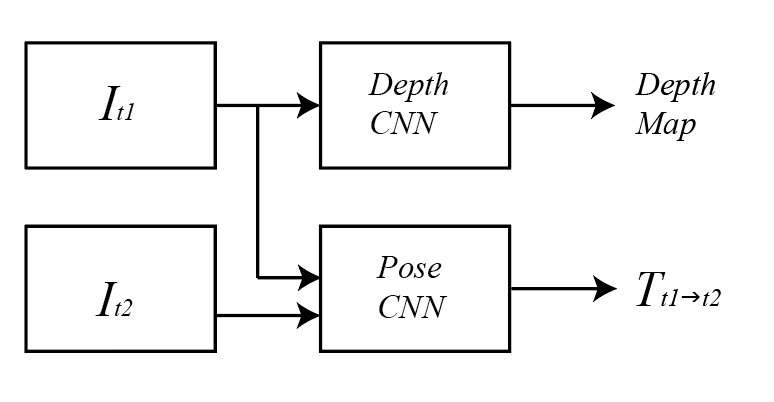
\includegraphics[width=3in]{images/cnns.png}
    \caption{Machine learning approaches have demonstrated strong results in simultaneously estimating depth maps and relative poses between images. Typically, a pair of CNN's is used, one for each task. The depth CNN is provided with the first view at $t=1$ and the pose CNN is provided both views.}
    \label{2cnns}
\end{figure}


While the training pipeline is unsupervised in the sense that labelled data is not required, some form of supervision signal is nevertheless required to optimise the parameters of the pair of networks. These papers take advantage of the fact that if the physical structure of a scene is known, then a novel rendering of that scene from a different viewpoint is achievable. Thus, \cite{garg2016unsupervised} suggested using photometric reconstruction as a supervision signal - from $I_{t2}$, reconstruct $I_{t1}$. The difference between the reconstruction and the real image can form a supervisory signal for the pair of networks. This work similarly uses photometric reconstruction as the principal supervisory signal in training a pair of networks to perform visual odometry and depth estimation. The photometric reconstruction loss is


\begin{equation}
    L_{photometric} = \sum_n^W \sum_m^H |I_{t1}(m,n) - \hat{I_{t1}}(m,n)|.
    \label{photometricloss}
\end{equation}


Humans can easily imagine what a scene will look like if we move our heads slightly, but only if we know the overall shape of the object we are looking at. Similarly, given two images separated by a small interval of time $I_{t1}$ and $I_{t2}$, one could synthesise what $I_{t1}$ would look like by sampling the pixels from $I_{t2}$, if the relative pose $T_{t1\rightarrow t2}$ between the two cameras and a pixel-wise depth of the scene $D_{t1}(p)$ is known. In practice, this can be done by obtaining the coordinates of the pixels in the first image $p_{t1}$ projected on to $I_{t2}$'s camera sensor. Assuming a pinhole model, the complete expression for $p_{t1}$'s projected location on the second camera, $\hat{p_{t2}}$ is 

\begin{equation}
\hat{p_{t2}} = KT_{t1\rightarrow t2} D(p_{t1}) K^{-1} p_{t1}.
\end{equation}

Here K represents the intrinsics matrix. In right-to-left order, this transform first maps each pixel to a ray direction using the inverse camera intrinsics $K^{-1}$. Each ray is then given a depth with the per-pixel depth map $D(p_{t1})$, producing a 3D point cloud. The transform $T_{t1 \rightarrow t2}$ transforms each point to the coordinate frame of the second camera, then the matrix $K$ projects each of those points onto the camera sensor of the second camera. The obtained coordinate $\hat{p_{t2}}$ is continuous, while pixel coordinates are discrete. A pixel value thus needs to be interpolated, keeping in mind that each step of a neural network pipeline must be differentiable to support the backpropagation of gradients. 

It was suggested by Zhou et al. \cite{zhou2017unsupervised} that adopting bilinear sampling could be used as a fully differentiable sampling mechanism. The use of bilinear interpolation as a differentiable sampling pipeline was first proposed Jaderberg et al. \cite{jaderberg2015spatialtransformer}, and adapted by Zhou et al. \cite{zhou2017unsupervised} to perform the differentiable image warp. A bilinear sampling kernel is described by 

\begin{equation}
    V = \sum_n^W \sum_m^H U_{nm} max (0, 1-|x - n|) max(0, 1-|y - m|).
\end{equation}

$V$ is the output of the sampling kernel, $U$ is the source image being sampled, $n$ and $m$ index over the columns and rows of the kernel respectively, $H$ and $W$ are the height and width of the sampling kernel, and $x$ and $y$ are the local coordinates of the sampling location. The $2 \times 2$ sampling kernel used to perform the photometric reconstruction is, in essence a weighted sum of the 4 nearest neighbour pixels, based on its proximity to those pixels. The equation is differentiable with respect to both x and y:


\begin{equation}
    \frac{\partial{V}}{\partial{x}} = \sum_n^W \sum_m^H U_{nm} max(0, 1-|y - m|).
\end{equation}
\begin{equation}
    \frac{\partial{V}}{\partial{y}} = \sum_n^W \sum_m^H U_{nm} max(0, 1-|x - n|).
\end{equation}

Using this bilinear sampling kernel, we can thus sample pixels from $I_{t2}$ to reconstruct $I_{t1}$ in a fully differentiable manner, allowing the backpropagation of gradients through the networks. The pipeline with photometric reconstruction as the supervision signal can be illustrated as shown in Figure \ref{supervisedMLCNNS}. Bilinear interpolation is similarly employed in this work to compute the photometric reconstruction loss of the estimated depth and pose. However, because this work operates on light fields, the output of photometric reconstruction won't be a single image, but a whole array of images.


\begin{figure}
    \centering 
    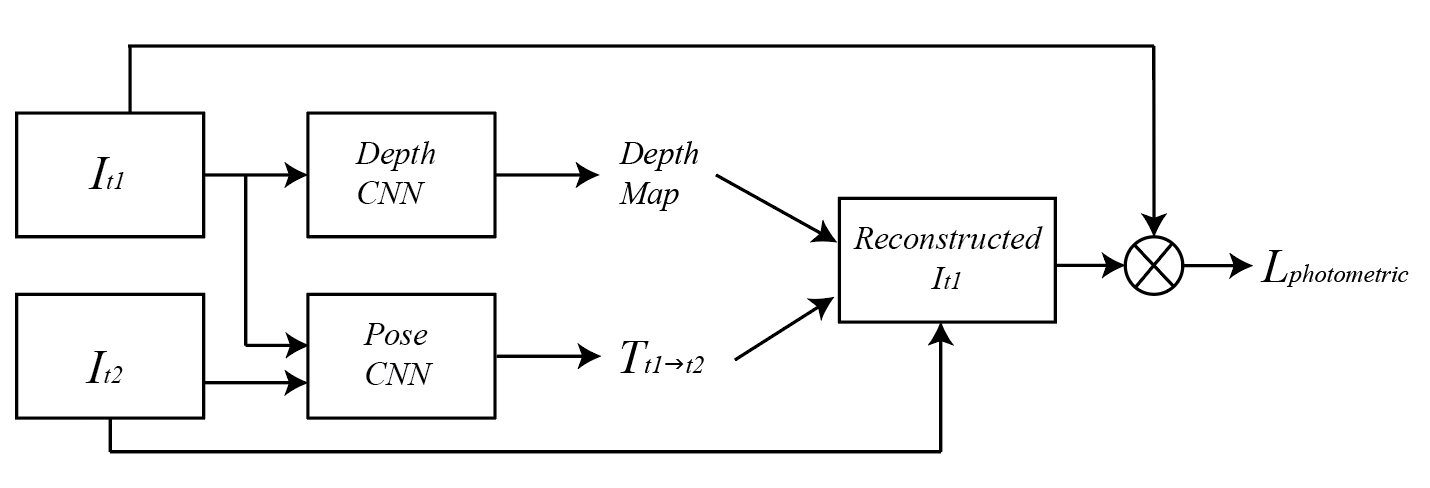
\includegraphics[width=5in]{images/mlpipeline.png}
    \caption{To provide a supervisory signal to the depth and pose CNN's, Garg et al. \cite{garg2016unsupervised} suggested using photometric reconstruction. The loss function is formulated by taking the difference between the reconstructed image $\hat{I_{t1}}$ and the actual image $I_{t1}$, shown in equation \ref{photometricloss}.}
    \label{supervisedMLCNNS}
\end{figure}


In addition to the photometric reconstruction loss providing the main supervision signal to the network, Zhou et al. \cite{zhou2017unsupervised} employs a smoothness loss to ensure that the produced depth map is globally smooth. The smoothness penalises the second order gradient of the image - i.e. the depth network is encouraged to produce a depth map characterised mostly by low-frequency components, and penalised for high-frequency components. Recognising that depth discontinuities frequently occur in parts of the image where a strong edge appears, Godard et al. \cite{godard2016consistency} on the other hand suggested the use of an edge-aware smoothness loss that also penalises large gradients in the depth map $\partial{d}$, but lowers the weight of the loss in regions where the image gradient $\partial{I}$ is large. 

\begin{equation}
    L_{smooth} =  \sum_n^W \sum_m^H |\partial_x d_{nm} e^{-|\delta_x I_{nm}|}| + \partial_y d_{nm} e^{-|\delta_y I_{nm}|}|
\end{equation}

There have been several iterations \cite{godard2016consistency, godard2018selfsupervised, zhan2018deepfeature} of this pipeline, most of which have focussed on introducing novel loss functions to improve the quality of the depth and pose estimates. To the best of our knowledge however, this pipeline has only ever been applied to monocular and stereo camera setups. While monocular and stereo cameras are ubiquitous in modern digital devices, this thesis will investigate the potential for the use of this pipeline to achieve improved results using a broader, more generalised family of imaging devices. 

Breaking free of the pinhole principle from which human eyes have developed and which commercial cameras have adopted, has wide implications in the field of machine vision. Reinforcing this idea is the rise in popularity of imaging techniques such as multi-spectral imaging, plenoptic cameras and polydioptric cameras, however interpreting ray directions and geometry for new cameras may not always be apparent, giving rise to the data-driven approach. Working on the principle that machine vision does not necessitate mimicking the human eye to capture imagery, this thesis investigates the capabilities of machine learning for querying depth and visual odometry using one such novel imaging device - a camera array.



\section{Convolutional Neural Networks and Light Field Images}

In order to craft such a machine learning pipeline that complements the use of camera arrays, an investigation into input methods for 4D light fields into convolutional neural networks is due. It is recognised in Sun et al. \cite{sun2016lfdepthcnn} that while epipolar plane images (EPI) explicitly encode depth information, directly extracting such information without significant post-processing refinement and computational cost is difficult. The literature demonstrates strong results in using a CNN to interpret the gradient-depth relationship between an EPI and the images corresponding depth map. An EPI is extracted in both the horizontal and vertical direction for every row and column of the image in the $u, v$ plane, and subsequently fed to the network as two long, cubic volumes to obtain their results.

The rich textural data available in a 4D lightfield was purposed by Wang et al. \cite{wang2016lfcnn} for the task of material recognition using a deep CNN. In addition to reporting significantly improved material-recognition results (from 70\% to 77\% accuracy), \cite{wang2016lfcnn} proposes and compares a number of strategies for training on 4D images. One method that achieves strong results uses an angular filter, taking advantage of the 'angular resolution' that is gained by using a light field image over 2D images. The 4D light field image is first reshaped to form what is called a 'remap' image. To illustrate what a remap image looks like, a traditional 2D image is formed by discrete pixels, whereas a remapped 4D image on the other hand is formed of blocks of pixels, each block of size $h_a \times w_a$, formed by taking one pixel from each camera in the array. The result is a 2D image from which a 2D convolutional filter is able to learn features that indicate texture and parallax. While the remapping method achieved the best results, unfortunately such an arrangement of the image data does not make sense in the case of the camera array being used for this project as the cameras are arranged in a crosshair formation - 8 vertical cameras, 8 horizontal and 1 center image. The remapped image using this camera would comprise $17 \times 17$ blocks of mostly black pixels, producing a very inefficient representation of the data. 

Another method proposed in \cite{wang2016lfcnn}, albeit one that demonstrated lower accuracy than the angular filter method, was to concatenate images along their RGB channels prior to being fed to the network. The dimensionality of the image is quickly downsampled, and is thus a more computationally and memory efficient method than using angular filters, whilst still demonstrating improvement over 2D images. A potential improvement on this strategy that may prove useful in this work would be to use a dilated convolution, effectively opening the receptive field to a much larger area of the image without increasing computational complexity. Such a CNN would benefit from being able to sample a larger area of the image to recognise robust geometric features. 

These strategies each treat light field images as a volume of 2D images, and thus do not take full advantage of the 4D signal structures present in a light field. One possible improvement that might learn to more effectively utilise these 4D signals is to swap out the 2D convolutional filters typically used in image data for a 3D convolutional filter which is more commonly applied to video data. 

\chapter{Learning Depth and Visual Odometry from Light Fields}

In Chapter 3, we saw that previous work has produced a variety of approaches to depth estimation and visual odometry, using both data-driven and hand crafted solutions. In this chapter, a pipeline is presented that matches the pipelines seen in chapter 3 in appearance, but differs in the functionality and type of input data. The contributions of previous work focus on the use of monocular and stereo image data, while this chapter focuses on developing a pipeline that employs the full breadth of geometric information in a light field. The first section of this chapter describes the tools and methodologies of acquiring a suitable dataset, while the second part walks through the development of the pipeline used.

\section{Data Acquisition}

\subsection{Ground Truth Pose Data}

\begin{figure}[h]
    \centering 
    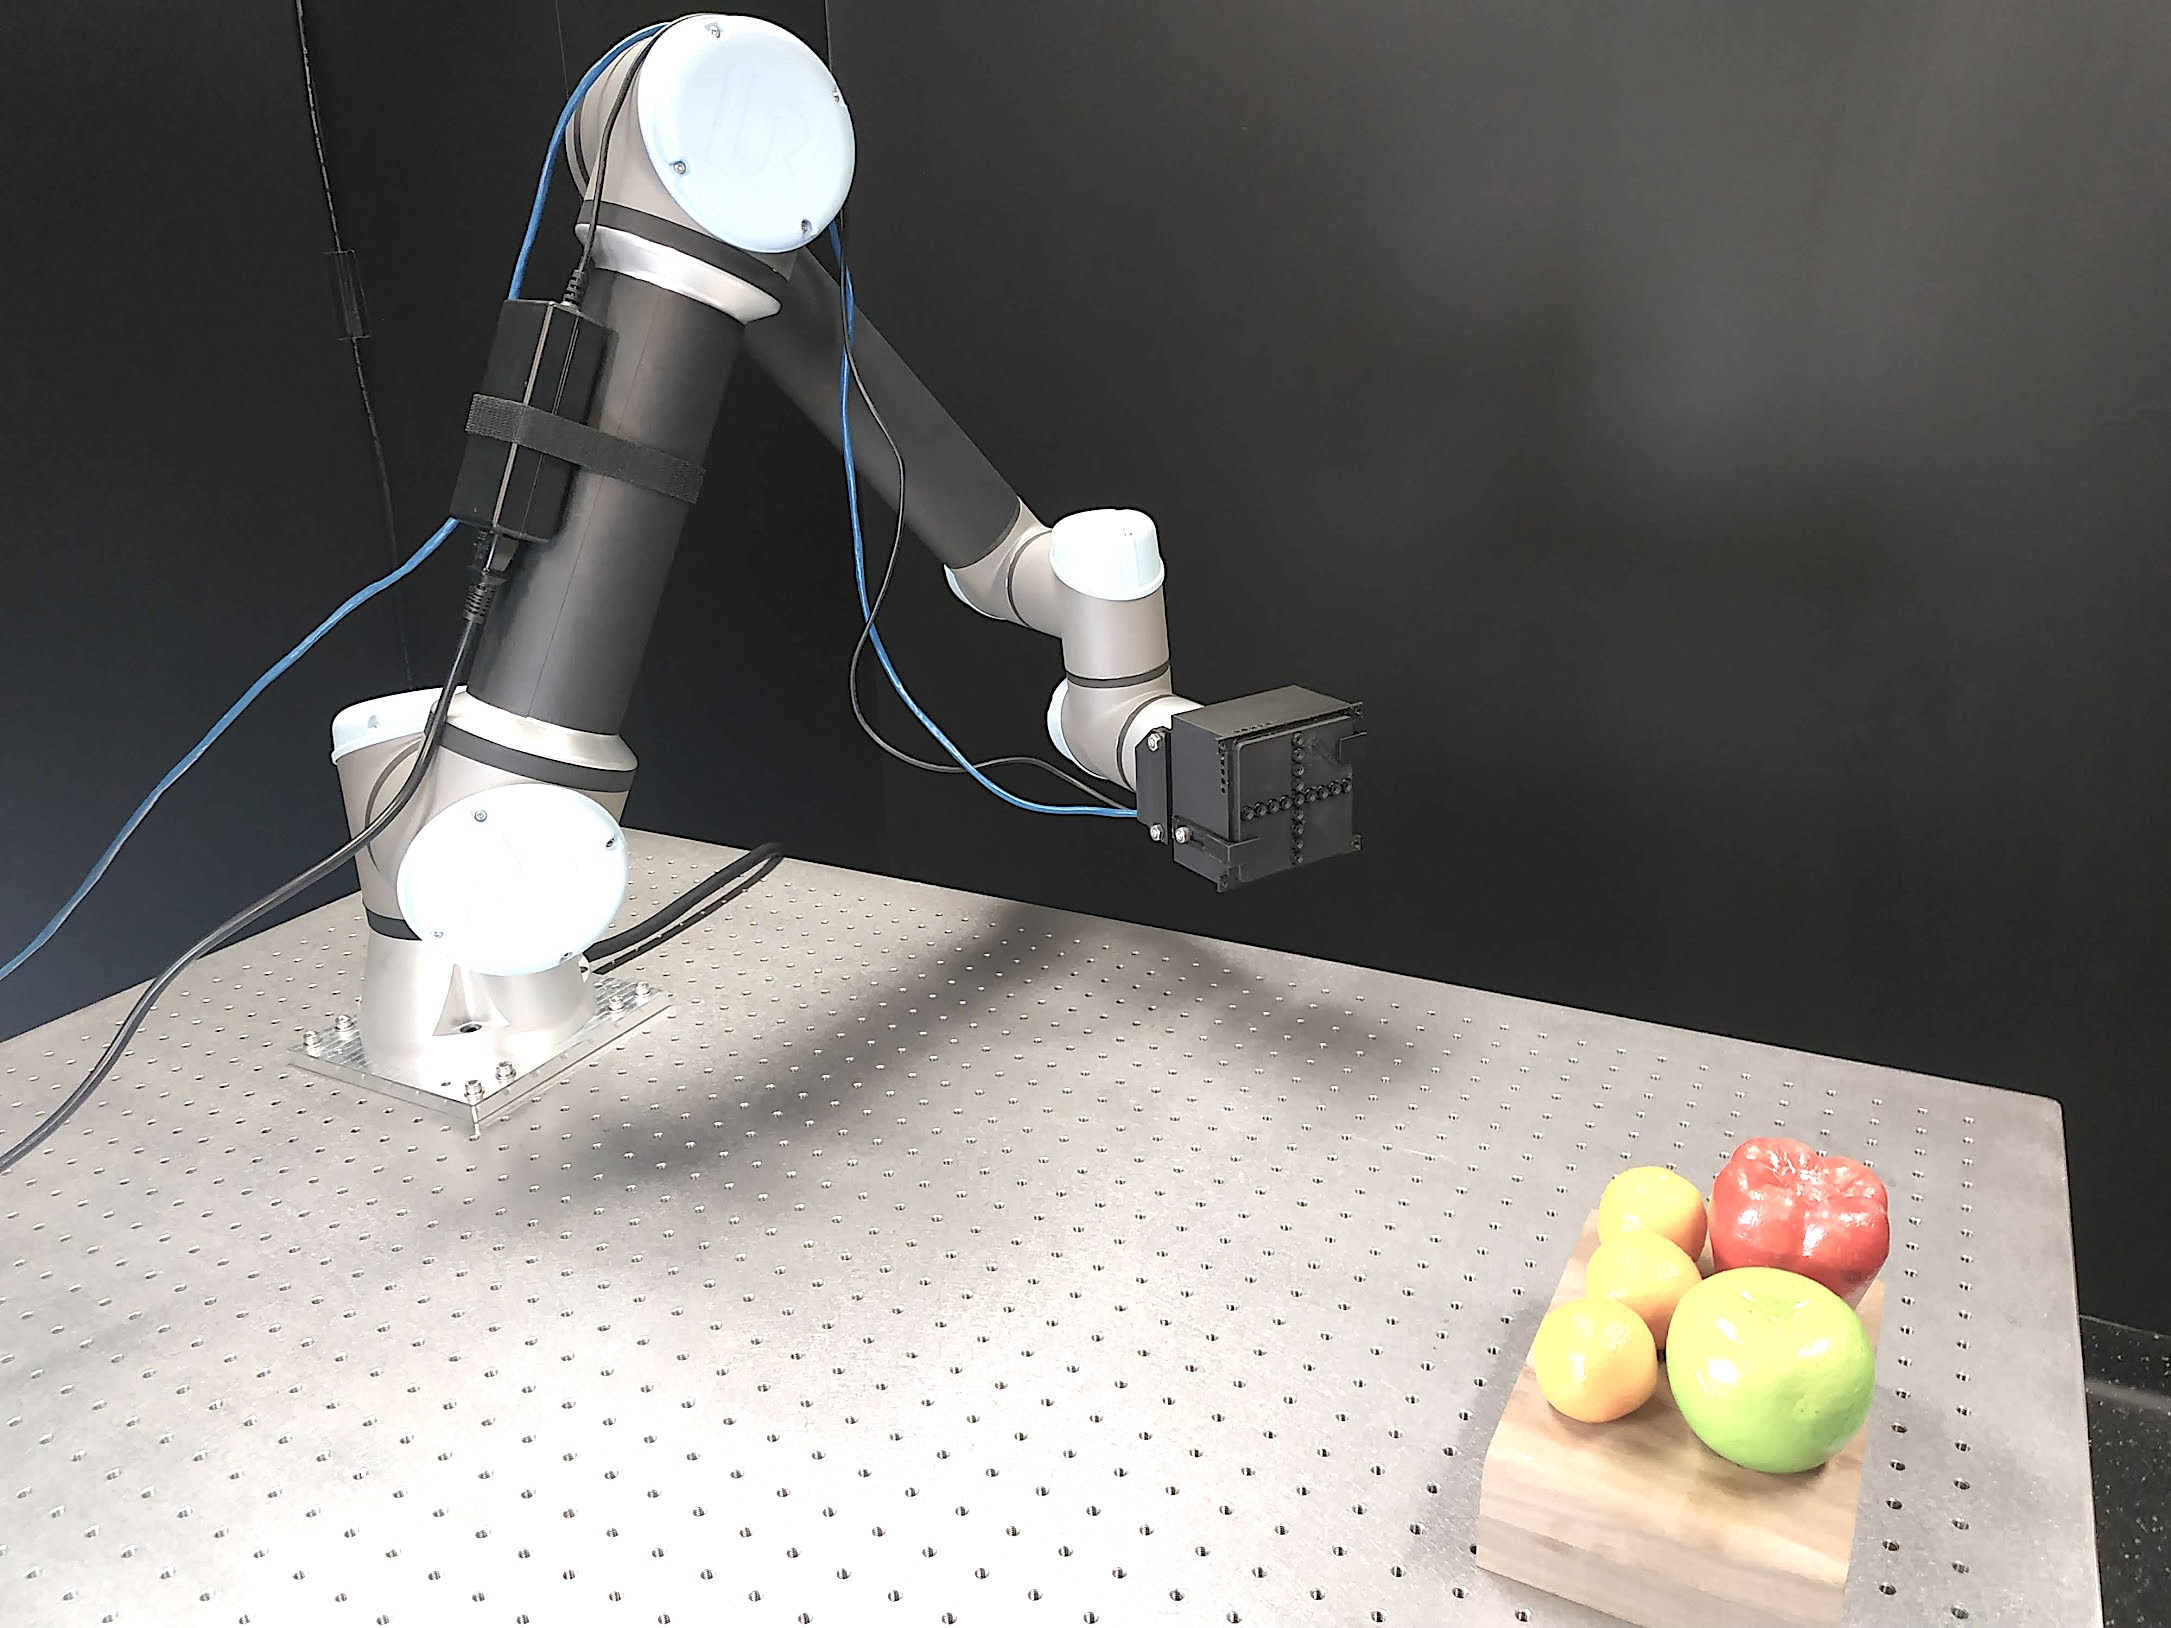
\includegraphics[width=4.5in]{images/experimentalsetup2.jpg}
    \caption{The experimental setup utilises a Universal Robots UR5E robotic arm to precisely measure ground-truth pose to allow effective evaluation of the projects visual odometry results.}
\end{figure}

Important to this work is a strong evaluation framework. Existing datasets such as KITTI and CityScapes benefit from state-of-the-art sensor suites including inertial sensors and lidar, allowing researchers to effectively benchmark their results. Similarly, this thesis places a strong emphasis on validation using ground truth data. One of the primary tasks for evaluation is visual odometry, and so ground-truth pose data for each image is a valuable resource. In this project, pose is collected by attaching the camera to a Universal Robots UR5E robotic arm, which is capable of sensing to a high degree of accuracy the pose of the end effector. Furthermore, the UR5E is able to perform accurate movements and trajectories with payloads of up to 5 kilograms, making it a suitable robotic mount for the camera. 

A challenge that needed to be solved prior to data collection was thus fabricating a rig for attaching the camera to the end effector. The UR5E uses a standard interface plate for attaching end-effectors such as grippers and other tools. The camera on the other hand, as an early prototype, does not have any suitable mounts available on the market for attaching it to the robot. A suitable mount therefore needed to be fabricated, taking into consideration the cameras ventilation and electronic connection requirements. A two-piece mount was designed using SolidWorks, and fabricated using fused deposition modelling (FDM) with polylactic acid (PLA) filament, allowing easy mounting and dismounting to the robot using standard M6 bolts. 

A client library for communicating with the UR5E was written in python, which establishes a TCP/IP connection with the robot over the local network, allowing both movement commands to be sent to the robot, and feedback data about the end-effector's pose to be streamed back to the client PC. The client library also provides functionality for pre-computing trajectories and joint angles, using the PyBullet physics engine and the known kinematic model of the robot. One useful trajectory function from the client library procedurally generates new waypoints with a stringent collision-checking mechanism, meaning data-collection can be performed autonomously. A challenge that has prevented a fully autonomous footage collection routine has been working with non-timestamped image data. The particular imaging setup currently provides only enough bandwidth for image data at roughly 1 frame every 2 seconds. Furthermore, the onboard rectification processes take several seconds to complete, and what's more, because the on board storage of the camera is limited, the image must be streamed over an ethernet connection to a PC taking several more seconds. The actual time that the image is captured is therefore ambiguous and so correlating each image with a pose-stamp is difficult. An intermediate solution has been to manually control the arm to each waypoint, and pausing while an image is taken and the pose is saved. 

\subsection{Imagery}

The specific imaging device being used is manufactured by EPIImaging, and consists of 17 subapertures. The communication interface with the camera is a network connection serving image data over the HTTP protocol via a straightforward URL request. Both rectified and unrectified images can be requested, and the format of the returned image data is a $17\times 3 \times 1280 \times 960$ block of bytes representing pixel data from each of the 17 image sensors. A simple client library was written in python that automates the URL request, and subsequent decoding of image bytes, allowing data to be collected quickly and conveniently.


\section{Depth and Visual Odometry Pipeline}

\begin{figure}[htbp]
    \centering 
    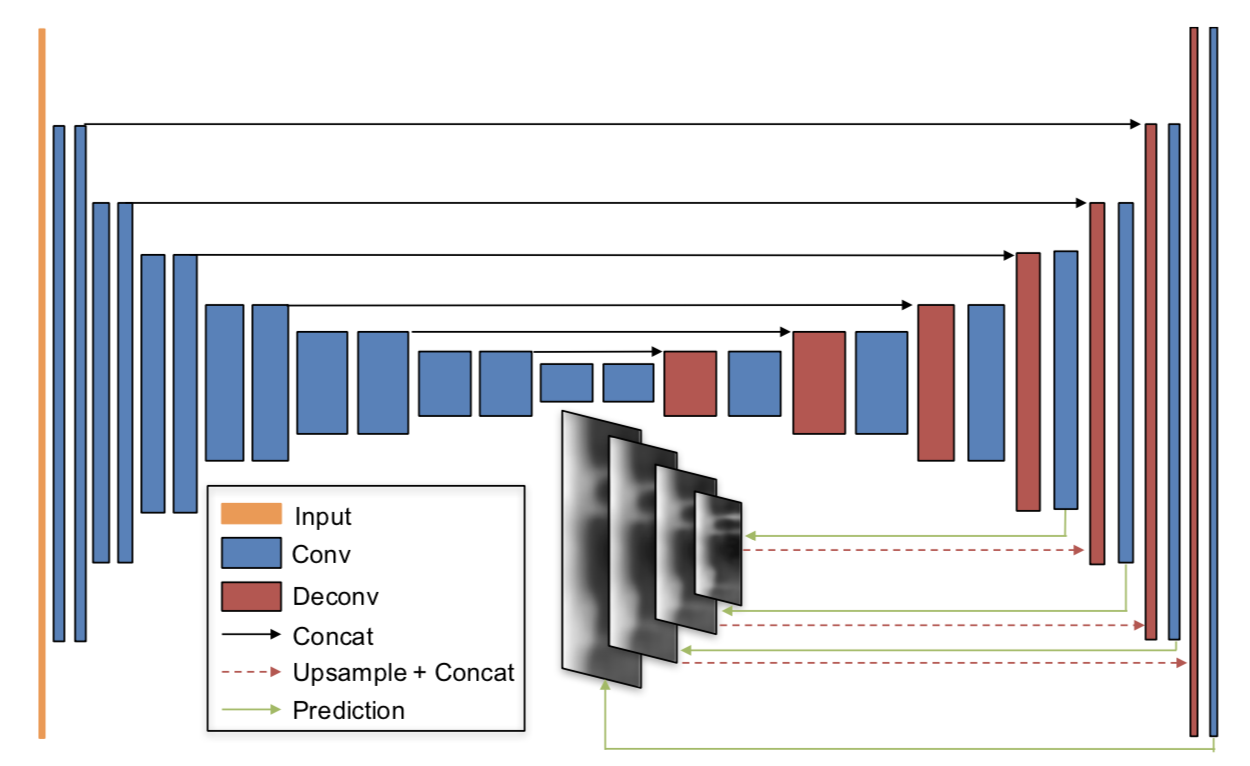
\includegraphics[width=2.5in]{images/dispnet.png}
    
\includegraphics[width=0.5in]{images/blank.png}
    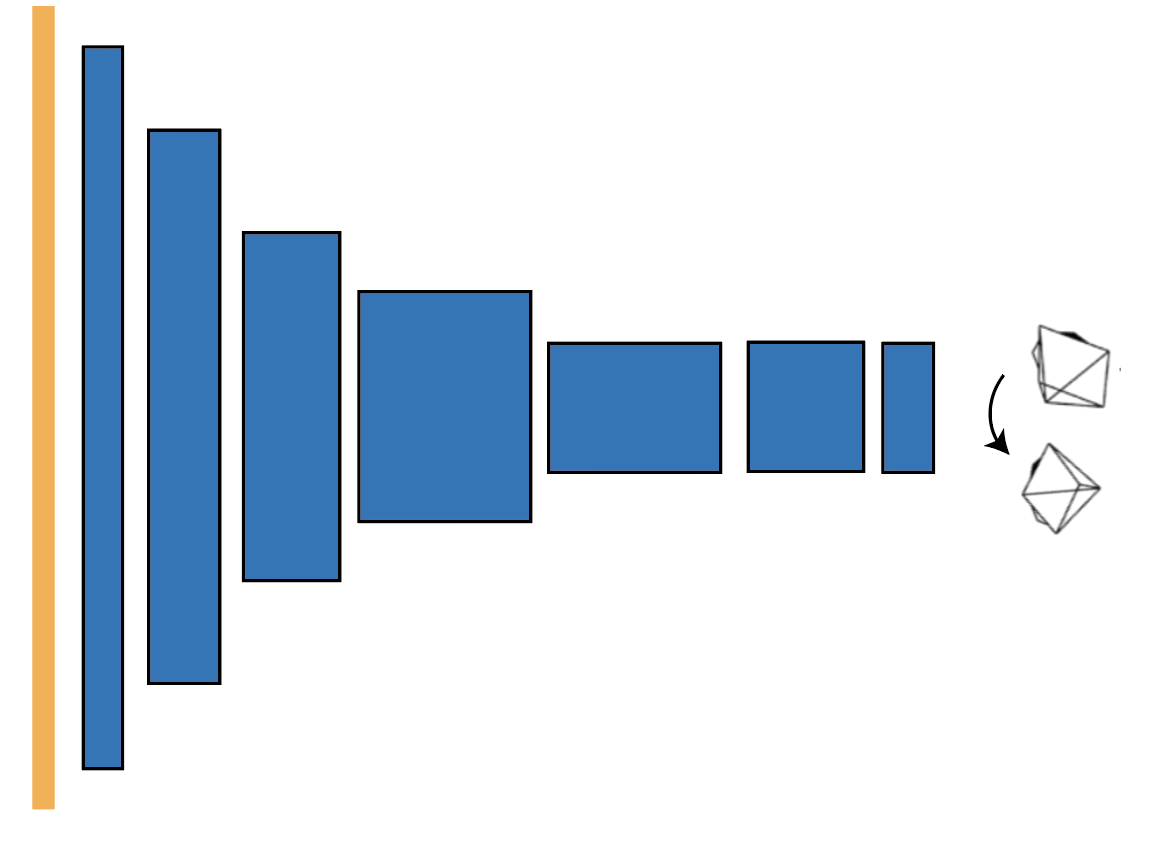
\includegraphics[width=2in]{images/posenet.png}
    \caption{(Left) The DispNet architecture uses a convolution encoder-decoder network characterised by skip connections, and outputs predictions at multiple scales. The multi-scale predictions aid in handling low-texture regions of the image. (Right) The PoseNet architecture uses a series of convolutional downsampling operations, predicting a final 6 degree-of-freedom pose estimate at its output activations.}
 \end{figure}

\subsection{Pose Estimation}

Estimating the 6-degree-of-freedom pose between two frames is treated as a regression problem, estimating three translational components [X, Y, Z] and three rotational components [Rx, Ry, Rz]. Importantly, the translation and rotation are regressed relative to the \textit{camera} coordinate frame of the first image, whereas the UR5E returns absolute position and orientation in the \textit{world} coordinate frame. The data preprocessing pipeline is thus required to compute the relative translation $P_{t1 \rightarrow t2}$ and rotation $R_{t1 \rightarrow t2}$ of two images, given their absolute positions $P_{t1}, P_{t2}$ and orientation $R_{t1}, R_{t2}$ in world coordinates. Concatenating translation and rotation into a single transform matrix $T = [R|t]$ allows us compute both relative rotation and translation in a single step, as:

\begin{equation}
T_{t1 \rightarrow t2} = T_1^{-1} T_2.
\end{equation}

The transform matrix can subsequently be decomposed into 3 translational and 3 rotational components. 

Regression of pose values is done with a CNN. As described in Chapter 2, there have been a variety of methods proposed for feeding light field images to CNNs. As of now, experiments have been conducted using light fields formatted as a stack of images concatenated along their colour channels. The two light fields are subsequently fed to the CNN, which produces 6 output values corresponding to the 6 degrees of freedom. The 'rectified linear unit' non-linearity function (ReLU) is used as an activation layer following each convolutional layer except the output prediction layer. 


\subsection{Depth Estimation}

Depth estimation is similarly modeled as a regression problem, with the same number of outputs as inputs. The depth estimation module uses a convolutional encoder-decoder architecture called DispNet as proposed in \cite{mayer2015dispnet}. Skip connections from the encoder to the decoder mean the decoding layers are able to access both high level features and low level features on either side of the latent space.

% \begin{figure}[htbp]
%     \centering 
%     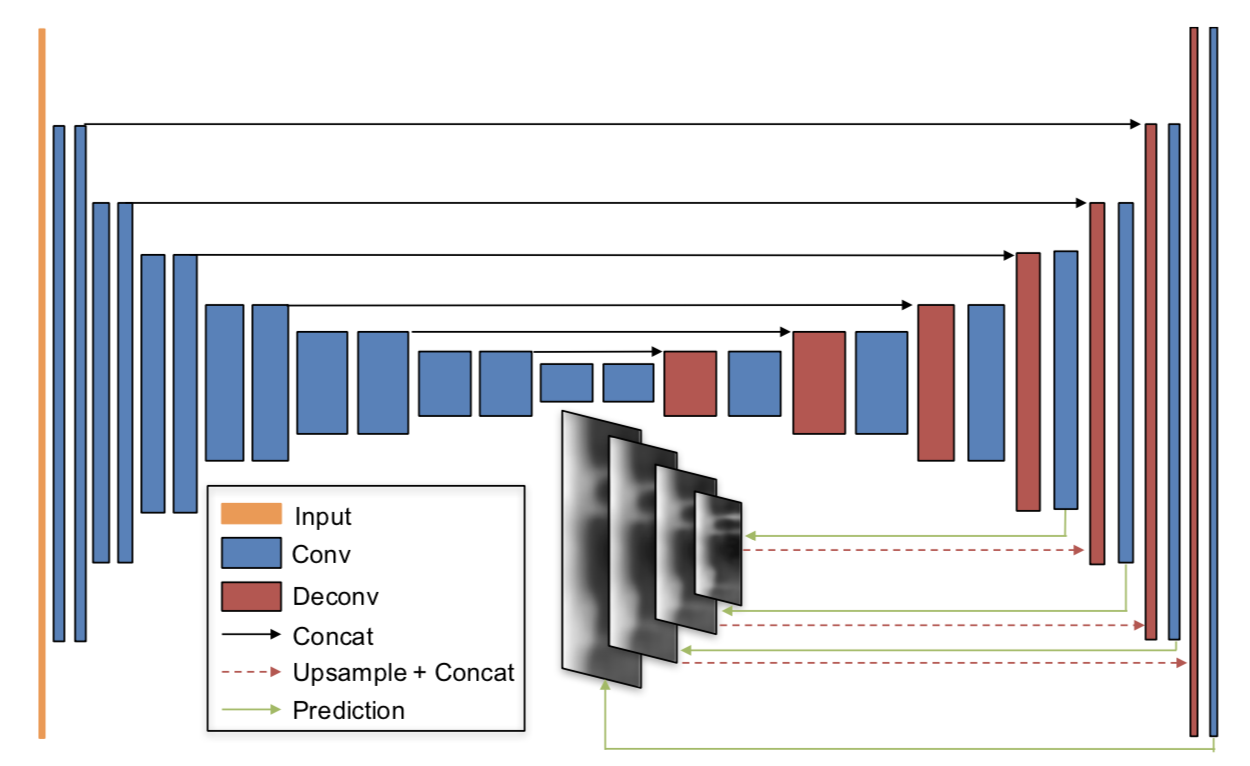
\includegraphics[width=3in]{images/dispnet.png}

%     \caption{The DispNet architecture uses a convolution encoder-decoder network characterised by skip connections, and outputs predictions at multiple scales. The multi-scale predictions aid in handling low-texture regions of the image.}
%  \end{figure}




\subsection{Differentiable Image Based Rendering}

Using the outputs from the depth and pose estimation modules, bilinear interpolation is used to photometrically reconstruct the first light field from the second. As described in Chapter 3, the procedure for this is to first project each pixel from $LF_1$ to a 3D point cloud using the known camera intrinsics and estimated depth values. Picking a single pixel $p1 = [s,t,u_1,v_1,1]^T$ from the first light field, and its corresponding depth estimate $D(p1)$, its projected point in 3D space is

\begin{equation}
    Q_{p1} = D(p1) K^{-1}[u_1,v_1,1]^T.
\end{equation}

The 3D coordinate $Q_{p1}$ can then be projected onto the camera sensor of $LF_2$, at the pixel coordinate $p_2 = [s,t,u_2,v_2]$. This relies on knowing the rigid transform $[R|T]$ from the first to the second camera origin.

\begin{equation}
    p_2 = K[R|t]Q_p.
 \end{equation}

This transform is equivalent to asking the question: knowing the depth of a pixel in image 1, where is the equivalent pixel in image 2? This procedure can be repeated for every pixel, allowing image 1 to be reconstructed entirely from the pixels of image 2. However, because pixels have discrete coordinates, and because we might find that the procedure described in equations 4.2 - 4.3 does not always produce an integer coordinate, the actual pixel value needs to be interpolated. The bilinear sampling kernel described in equations 3.3 - 3.5 is used as a differentiable method that supports backpropagation of errors. 

The supervision signal for the network is the sum of the photometric reconstruction loss (equation 3.1), and the regularising edge-aware smoothness loss (equation 3.2)

\begin{equation}
    L = L_{photometric} + L_{smooth}.
\end{equation}



\section{Experiments: Supervised Visual Odometry}

A simple, yet revealing experiment is to train a model to perform visual odometry in a fully supervised setting. While unsupervised methods form a supervision signal by cleverly piecing together the available information, a fully supervised approach on the other hand theoretically produces the best possible results for any given system. Thus, there is a motivation to test the performance of the neural architectures described above. Not only does this experiment uncover what the pose network is capable of, but the experiment lays the groundwork for future unsupervised experiments. Individual modules such as the network itself, the data-loading module and even the weights of the trained network \footnote{While using pretrained weights to reduce training time is common practice, care is taken in this work to avoid using overlapping datasets when using pretrained weights. The dataset used to supervise the pre-trained weights should not contain the same scenes used to train the unsupervised model.} can be reused in future experiments. 

\subsection{Monocular Visual Odometry}

In the first iteration of this experiment, the KITTI dataset is used thanks to the size of the dataset and the availability of ground truth pose measurements. The input to the network is the pair of images in the sequence, and the loss function is computed from the ground truth 6-degree-of-freedom pose transform from one frame to the next. Evaluation is performed on sequences of the KITTI dataset that were withheld at training time, so as to gain an understanding of the models ability to generalise outside of the training data. 

The network was trained for 18 hours, completing 70 passes over the input dataset. Stochastic gradient descent was used as the optimisation algorithm, using batch sizes of 8 images. The network was trained with pairs of image in both forwards and reverse order, meaning the network had to learn to predict both forwards and backwards motion. Input images were normalised with a mean pixel value at zero over the entire dataset, and divided by the standard deviation of the dataset. 


\begin{figure}[htbp]
    \centering
    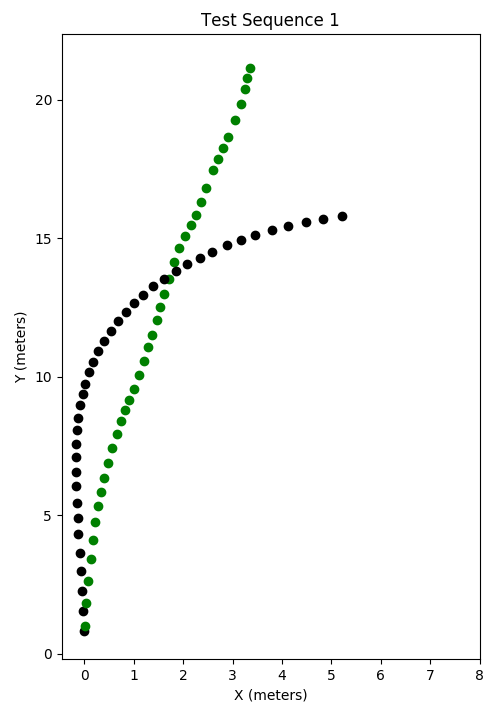
\includegraphics[height=2.4in]{images/vo_results/0034.png}
    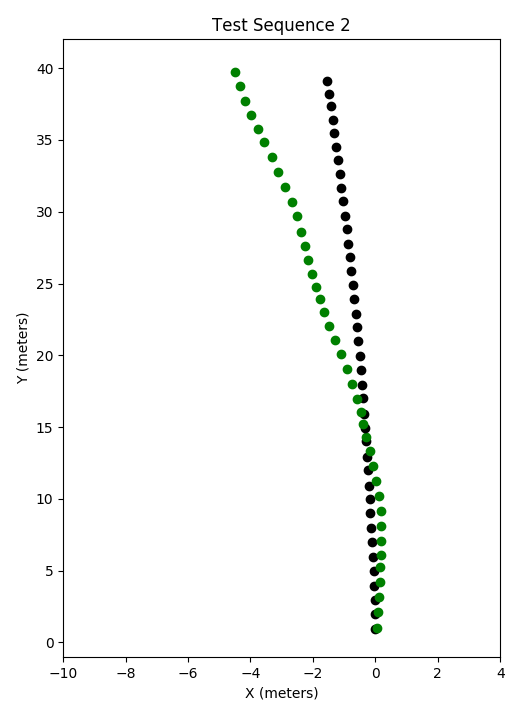
\includegraphics[height=2.4in]{images/vo_results/0018.png}
    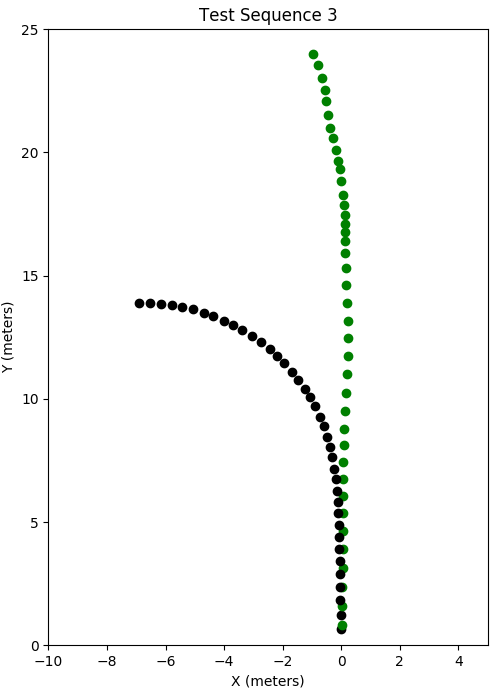
\includegraphics[height=2.4in]{images/vo_results/0027.png}
    
\includegraphics[height=0.2in]{images/vo_results/legend.png}

    \caption{Examples of trajectories generated from ground truth and estimated poses. These trajectories are generated over snippets of 40 frames from three test sequences which were withheld during training of the model. The cumulative nature of the error becomes more apparent the further the vehicle strays from the origin.}

    \label{vo_results_kitti}
    
\end{figure}

\begin{table}[tbp]

    \caption{Summary of Results for three test sequences}
    \centering
    \begin{tabular}{@{}llll@{}}
        \toprule
        Measure            & Sequence 1    & Sequence 2   & Sequence 3  \\ \midrule
        Frames             & 40            & 40           & 40          \\
        Path Length (m)    & 18.28         & 39.14        & 17.58       \\ \midrule
        \multicolumn{4}{l}{Instantaneous Translational RMS Error (m)}   \\
        X                  & 0.129         & 0.101        & 0.181       \\
        Y                  & 0.013         & 0.034        & 0.018       \\
        Z                  & 0.193         & 0.081        & 0.277       \\ \midrule
        \multicolumn{4}{l}{Absolute Trajectory RMS Error (m)} \\
        X                  &  0.81         & 1.39         & 2.70        \\
        Y                  &  2.17         & 0.24         & 5.42        \\
        Z                  &  0.12         & 0.37         & 0.25        \\ \bottomrule
    
        \end{tabular}
        \label{kitti_vo_results_tabular}
    \end{table}



Some examples of trajectories generated using raw-ground truth data and the predicted trajectories over 40 frame snippets of video are shown in Figure \ref{vo_results_kitti}. Because the trajectory of a vehicle driving along a road can be described almost entirely by its movements in a 2D plane, these trajectories are plotted as such, ignoring the minor up and down motions of the vehicle. While the error grows and becomes more evident at larger distances from the origin, the individual frame-to-frame error is qualitatively small. In observing these trajectories, we also note that while the network appears to have modeled forward and linear motion quite well, rotation seems to have been left behind. 

Results from the experiment are reported in Table \ref{kitti_vo_results_tabular}. The table summarises the instantaneous translational errors from frame to frame as well as the absolute pose error of the cumulative trajectory. These errors are computed as the root-mean-square error of the distance between the predicted and ground truth poses for the 3 translation components. In this table, instantaneous translational errors are reported relative to the X-Y-Z coordinate frame of the camera (Z pointing out through the lens), while the absolute trajectory error is reported relative to the coordinate frames shown in Figure \ref{vo_results_kitti}.







We observe in the tabulated results that the pose prediction consistently performs best in predicting translation in the $Z$ direction (up and down relative to the road). This is expected, as a vehicle driving on a flat road is likely to experience minimal up-and-down motion relative to the forwards-backwards and side-to-side components. The $Z$ translation of the cost function can thus be minimised easily by consistently predicting zero, or very close to zero for that component. Forwards and backwards instantaneous translations were predicted best in sequence two - a relatively straight stretch of road. This is indicative of the models difficulty when faced with tight corners as shown in sequences 1 and 3. 

\subsection{Plenoptic Visual Odometry}
A seemingly simple extension of the experiment described in the previous section is to perform the same procedure using light field imagery. With improved exposure to depth information, the model should see an improvement in performance, particularly in the awareness of scale. By providing multiple views, the model is able to implicitly learn the geometric features associated with the unchanging baseline between sub-apertures. This will aid in accurately predicting the magnitude of the rotations and translations in space. Such a model can learn to employ more robust features such as parallax and occlusion to estimate motion with improved scale awareness. After all, in the monocular case, the model must learn to infer scale from features of the scene (height above the ground or knowledge of the rough size of pedestrians could be features used by the model to make its predictions). 

While the pose network is capable of ingesting light field imagery and a small dataset is ready for training with, experiments thus far have yielded numerically unstable training losses, even in the case of single sub-apertures - an effectively identical approach to the experiment described in the previous section. An investigation is currently underway into the reasons behind this instability. 


\chapter{Updated Research Proposal}

As this thesis project approaches the half-way point, it is worth updating the original research proposal to reflect the projects current progress and timeline. 16 weeks have passed since the beginning of the project, and 25 weeks remain before the seminar presentation in week 13 of semester 1 2020.

\section{Milestones}

\subsubsection{Data Acquisition}
Achieving a critical mass of data is an important milestone in this project, as it is heavily reliant on an abundance of training data. The majority of data collection activities are expected to be completed within the next two weeks, with a view to collecting 10,000 pose-stamped light field images. 

\subsubsection{Algorithm Development and Evaluation}
This thesis proposes a fully-unsupervised depth and visual odometry pipeline. On the path to achieving this algorithm however, is a number of useful experiments that can be performed to gather preliminary results and prepare for challenges in the final formulation of the centerpiece algorithm. One of these experiments is described in chapter 5 - using ground truth pose data to supervise a visual-odometry-performing CNN. 

The most important milestone currently being worked towards for the algorithm and software development part of this thesis is understanding the root cause of the numerical instability seen in training the model when using light field imagery. Chapter 5 demonstrated that visual odometry is absolutely possible using CNN's. I therefore firmly believe that there is likely to be an error in interpreting pose stamps collected from the robot arm, rather than the nature of the task itself being too difficult for a network to solve. This experiment will be completed and delivered in the next 4 weeks, by which time an evaluation study will be written with results and discussion. 

Once this supervised CNN is demonstrated to properly ingest light field imagery and produce pose estimates, work will begin on inserting the depth estimation module into the pipeline. Many of the components of the depth estimation module are already in place, ready to be added to the pipeline. This will be completed in the next 12 weeks. Once the algorithm is demonstrated to work in the most simple cases, there will be a three main experiments to perform. 

The first will experimentally evaluate different methods of feeding light field imagery to convolutional neural networks. The second will experimentally determine the differences in performance when different numbers of sub-apertures from the camera array are used. A full validation study surrounding this component of the thesis will be produced in the next 16 weeks. 

A comfortable buffer is built into this plan to allow for the expected decrease in time available for this project once the semester begins in February 2020. 

\subsubsection{Preparation of Seminar Materials and Final Thesis Submission}
The remainder of the time available for this thesis project will be devoted to preparing materials for the seminar presentation and final thesis submission. I expect that a large amount of this time will still be spent collecting results and making experimental changes to the pipeline, but large structural changes to the program will be avoided. 

\newpage

%\newpage
\bibliographystyle{plain}
\bibliography{bibliography.bib}

\end{document}
